%% LyX 2.1.4 created this file.  For more info, see http://www.lyx.org/.
%% Do not edit unless you really know what you are doing.
\documentclass[a4paper,english]{article}
\usepackage[osf]{mathpazo}
\renewcommand{\sfdefault}{lmss}
\renewcommand{\ttdefault}{lmtt}
\usepackage[T1]{fontenc}
\usepackage[latin9]{inputenc}
\usepackage{amsmath}
\usepackage{amssymb}

\makeatletter

%%%%%%%%%%%%%%%%%%%%%%%%%%%%%% LyX specific LaTeX commands.
\pdfpageheight\paperheight
\pdfpagewidth\paperwidth

%% Because html converters don't know tabularnewline
\providecommand{\tabularnewline}{\\}

%%%%%%%%%%%%%%%%%%%%%%%%%%%%%% User specified LaTeX commands.
\usepackage{tikz}
\usetikzlibrary{matrix,arrows,decorations.pathmorphing}
\usetikzlibrary{shapes.geometric}
\usepackage{tikz-cd}
\usepackage{amsthm}
\theoremstyle{plain}
\newtheorem{theorem}{Theorem}[section]
\newtheorem{lemma}[theorem]{Lemma}
\newtheorem{prop}{Proposition}[section]
\newtheorem*{cor}{Corollary}
\theoremstyle{definition}
\newtheorem{defn}{Definition}[section]
\newtheorem{ex}{Exercise} 
\newtheorem{example}{Example}[section]
\theoremstyle{remark}
\newtheorem*{rem}{Remark}
\newtheorem*{note}{Note}
\newtheorem{case}{Case}
\usepackage{graphicx}
\usepackage{amssymb}
\usepackage{tikz-cd}
\usetikzlibrary{calc,arrows}
\tikzset{mydot/.style={circle,fill,inner sep=1.5pt},
commutative diagrams/.cd,
  arrow style=tikz,
  diagrams={>=latex},
}

\usepackage{babel}
\usepackage{hyperref}
\hypersetup{
    colorlinks,
    citecolor=black,
    filecolor=black,
    linkcolor=black,
    urlcolor=black
}

\makeatother

\usepackage{babel}
\begin{document}

\title{Category Theory Course}


\author{John Baez}

\maketitle
\pagebreak{}

\tableofcontents{}

\pagebreak{}


\section{Category Theory:}
\begin{itemize}
\item Unifies mathematics.
\item Studies the mathematics of mathematics (similar to mathematical logic).
\item Moves towards higher-dimensional algebra (``homotopifying'' mathematics).
\end{itemize}
\begin{center}
\begin{tabular}{ccccccc}
 &  &  &  &  &  & \tabularnewline
\begin{tikzcd} \\ \\ \bullet && \bullet \\ & \bullet \\ \bullet  && \bullet \\ \\ \end{tikzcd} &  &  &  &  &  & \begin{tikzcd} \\ \\ \bullet \arrow[loop left] \arrow[dr] \arrow[rr, bend left] && \bullet \arrow[loop right] \arrow[dd, bend left] \arrow[dl] \\ & \bullet \\ \bullet \arrow[loop left] \arrow[ur] \arrow[uu, bend left] && \bullet \arrow[ll, bend left] \arrow[loop right] \arrow[ul] \\ \\ \end{tikzcd}\tabularnewline
Set Theory &  &  &  &  &  & Category Theory\tabularnewline
0-dimensional &  &  &  &  &  & 1-dimensional\tabularnewline
 &  &  &  &  &  & \tabularnewline
\end{tabular}
\par\end{center}

\pagebreak{}


\subsection{Definition of a Category}

A $\emph{category}$ $\mathbf{C}$ consists of: 
\begin{itemize}
\item A class $Ob(\mathbf{C})$ of $objects$. If $x\in Ob(\mathbf{C})$,
we simply write $x\in\mathbf{C}$.
\item Given $x,y\in\mathbf{C},$ there's a set $Hom_{\mathbf{C}}(x,y)$,
called a $\emph{homset}$, whose elements are called $\emph{morphisms}$
or $\emph{arrows}$ from $x$ to $y$. If $f\in Hom_{\mathbf{C}}(x,y)$,
we write $f:x\to y$. 
\item Given $f:x\to y$ and $g:y\to z$, there is a morphism called their
$\emph{composite}$ $g\circ f:x\to z$. 
\end{itemize}
\begin{center}\begin{tikzcd}[column sep=small] & y \arrow[dr,"g"] & \\ x \arrow[ur,"f"] \arrow[rr,"g \circ f" below] & & z \end{tikzcd}\end{center}
\begin{itemize}
\item Composition is associative: $(h\circ g)\circ f=h\circ(g\circ f)$
if either side is well-defined.
\end{itemize}
\begin{center}\begin{tikzcd} \bullet \arrow[dddrrr, "h \circ f" near end] \arrow[rrr,"g"] &&& \bullet \arrow[ddd,"h"] \\\\\\ \bullet \arrow[uuu,"f"] \arrow[uuurrr,"g \circ f" near start, crossing over] \arrow[rrr,"h \circ (g \circ f)=(h \circ g) \circ f" below] &&& \bullet \end{tikzcd}\end{center}
\begin{itemize}
\item For any $x\in\mathbf{C}$, there is an $\emph{identity morphism}$
$1_{x}:x\to x$ 
\end{itemize}
\begin{center}\begin{tikzcd} x \arrow[loop, "1_x" swap] \end{tikzcd}\end{center}
\begin{itemize}
\item We have the $\emph{left and right unity laws}$:
\end{itemize}
\begin{center}
$1_{x}\circ f=f$ for any $f:x'\to x$
\par\end{center}

\begin{center}
$g\circ1_{x}=g$ for any $g:x\to x'$
\par\end{center}


\subsection*{Examples of Categories}


\subsubsection{Categories of mathematical objects}

For any kind of mathematical object, there's a category with objects
of that kind and morhpisms being the structure-preserving maps between
the objects of that kind. 

\begin{example} $\mathbf{Set}$ is the category with sets as objects and functions as morphisms. \end{example}

\begin{example} $\mathbf{Grp}$ is the category with groups as objects and homomorphisms as morphisms. \end{example}

\begin{example} For any field $k$, $\mathbf{Vect}_k $ is the category with vector spaces over a field k as objects and linear maps as morphisms. \end{example}

\begin{example} $\mathbf{Ring}$ is the category with rings as objects and ring homomorphisms as morphisms. \end{example}

These are categories of ``algebraic'' objects, namely, a set ($\emph{stuff}$)
with operations ($\emph{structure}$) such that a bunch of equations
hold ($\emph{properties}$), with morphisms being functions that preserve
the operations. All this is formalized in ``universal algebra'',
using ``algebraic theories''. There are also categories of non-algebraic
gadgets:

\begin{example} $\mathbf{Top}$ is the category with topological spaces as objects and continuous maps as morphisms. \end{example}

\begin{example} $\mathbf{Met}$ is the category with metric spaces as objects and continuous maps as morphisms. \end{example}

\begin{example} $\mathbf{Meas}$ is the category with measurable spaces as objects and measurable maps as morphisms. \end{example}


\subsubsection{Categories as mathematical objects}

There are lots of small, managebable categories:

\begin{defn} A \emph{monoid} is a category with one object. \begin{rem}$Hom_{\mathbf{C}}(\bullet,\bullet)$ for this object $\bullet$, is a set with associative product and unit. \end{rem} \end{defn}

\begin{center}\begin{tikzcd} \bullet \arrow[loop right, "f"]  \arrow[loop left, "g"] \arrow[loop above, "1_\bullet"] \end{tikzcd}\end{center}

\begin{example} \begin{tikzcd} \bullet \arrow[loop right, "f"] \arrow[loop left, "1_{\bullet}"] \end{tikzcd} \end{example}

\begin{center}
\begin{tabular}{c|c|c}
$\circ$ & $1_{\bullet}$ & $f$\tabularnewline
\hline 
$1_{\bullet}$ & $1_{\bullet}$ & $f$\tabularnewline
\hline 
$f$ & $f$ & $1_{\bullet}$\tabularnewline
\end{tabular}
\par\end{center}

\begin{flushleft}
The multiplication table above tells us how to compose morphisms.
The resulting monoid is usually called $\mathbb{Z}/2\mathbb{Z}$.
Now, consider the same diagram but with this multiplication table
instead:
\par\end{flushleft}

\begin{center}
\begin{tabular}{c|c|c}
$\circ$ & $1_{\bullet}$ & $f$\tabularnewline
\hline 
$1_{\bullet}$ & $1_{\bullet}$ & $f$\tabularnewline
\hline 
$f$ & $f$ & $f$\tabularnewline
\end{tabular}
\par\end{center}

\begin{flushleft}
Here we get another famous monoid:
\par\end{flushleft}

\begin{center}
\begin{tabular}{ccccc}
$1_{\bullet}$ = true &  &  &  & $1_{\bullet}$ = false\tabularnewline
$f$ = false &  & or alternatively &  & $f$ = true\tabularnewline
$\circ$ = or &  &  &  & $\circ$ = and\tabularnewline
\end{tabular}
\par\end{center}

\begin{defn} A morphism $f:x\to y$ is an $\emph{isomorphism}$ if
it has an $\emph{inverse}$ $g:y\to x$, that is, a morphism with:

\[
g\circ f=1_{x}
\]
\[
f\circ g=1_{y}
\]


\begin{flushleft}
If there exists an isomorphism between two objects $x,y\in\mathbf{C}$,
we say they're $\emph{isomorphic}$. 
\par\end{flushleft}

\end{defn}

\begin{defn} A category where all morphisms are isomorphisms is called a $\emph{groupoid}$. \end{defn}  

\begin{example} "The groupoid of finite sets" is obtained by taking $\mathbf{FinSet}$, with finite sets as objects and functions as morphisms, and then throwing out all morphisms except isomorphisms (i.e. bijections).\end{example}

\begin{defn} A monoid that is a groupoid is called a $\emph{group}$. \begin{rem} the usual 
"elements" of a group are now the morphisms. \end{rem} \end{defn}

\begin{defn} A category with only identity morphisms is a $\emph{discrete}$ category. \begin{rem} So any set is the set of objects of some discrete category in a unique way.  So a discrete category is "essentially the same" as a set. \end{rem} \end{defn}

\begin{center}\begin{tikzcd} \bullet \arrow[loop, "1_{\bullet}" swap] && \bullet \arrow[loop, "1_{\bullet}" swap] \\\\ \bullet \arrow[loop, "1_{\bullet}" swap]  && x \arrow[loop, "1_{x}" swap] \end{tikzcd}\end{center}

\begin{defn} A $\emph{preorder}$ is a category with at most one morphism in each homset.\end{defn}

\begin{flushleft}
If there is a morphism $f:x\to y$ in a preorder, we say ``$x\leq y$'';
if not, we say ``$x\nleq y$. For a preorder, the category axioms
just say:
\par\end{flushleft}
\begin{itemize}
\item Composition: $x\leq y$ and $y\leq z$ $\implies$$x\leq z$. 
\item Associativity is automatic.
\item Identities: $x\leq x$ always.
\item Left and right unit laws are automatic.
\item We're not getting antisymmetry: $x\leq y$ and $y\leq x$ $\implies$
$x=y$.
\end{itemize}
\begin{defn} An $\emph{equivalence relation}$ is a preorder that's also a groupoid.\end{defn}

\begin{prop} A preoder is a groupoid if and only if this extra law holds for all $x,y \in \mathbf{C}$: \end{prop}

\begin{center}$x \leq y \implies y \leq x$\end{center}

\begin{flushleft}
Here we have transitivity, reflexivity, and symmetry of ``$\leq$''.
So we usually call this relation $\sim$.
\par\end{flushleft}

\begin{prop} A preorder is skeletal, i.e. isomorphic objects are equal, if and only if this extra law holds  for all $x,y \in \mathbf{C}$:  \begin{center}$(x \leq y) \wedge (y \leq x) \implies x=y$ \end{center}\end{prop}

\begin{flushleft}
In this case we say that $\mathbf{C}$ is a $\emph{poset}$. 
\par\end{flushleft}

\begin{example} Preorder that is a groupoid but not a poset: \end{example}

\begin{center}\begin{tikzcd} \bullet \arrow[loop left] \arrow[r, bend left] & \bullet \arrow[loop right] \arrow[l, bend left] && \end{tikzcd}\end{center}

\begin{example} Preorders that are posets but not groupoids: \end{example}

\begin{center}\begin{tikzcd} \bullet \arrow[loop left] &&\\ \bullet \arrow[u] \arrow[loop left] \\ \bullet \arrow[loop left] \arrow[u] \end{tikzcd} \begin{tikzcd}[column sep=small] \bullet \arrow[loop above] && \bullet \arrow[loop above] \\& \bullet \arrow[loop below] \arrow[ul] \arrow[ur] \end{tikzcd} \end{center}

\begin{example} Preorder that is both a poset and a groupoid: \end{example}

\begin{center}\begin{tikzcd} \bullet \arrow[loop] \end{tikzcd} \end{center}

\begin{flushleft}
Since categories can be seen as mathematical objects, we should define
maps between them:
\par\end{flushleft}

\begin{defn} Given categories $\mathbf{C}$ and $\mathbf{D}$, a $\emph{functor}$ $F:\mathbf{C} \to \mathbf{D}$ consists of: \end{defn}
\begin{itemize}
\item a function called $F$ from $Ob(\mathbf{C})$ to $Ob(\mathbf{D})$:
if $x\in\mathbf{C}$ then $\mathbf{F}(x)\in\mathbf{D}$.
\item functions called $F$ from $Hom_{\mathbf{C}}(x,y)$ to $Hom_{\mathbf{C}}(F(x),F(y))$,
for all objects $x,y\in\mathbf{C}$: if $f:x\rightarrow y$ then $F(f):F(x)\rightarrow F(y)$
\end{itemize}
such that:
\begin{itemize}
\item $F(g\circ f)=F(g)\circ F(f)$ whenever either side is well defined.
\item $F(\mathbf{1}_{x})=\mathbf{1}_{F(x)}$ for all $x\in\mathbf{C}$.
\end{itemize}
So a functor looks like this:

\begin{center}
\begin{tabular}{ccccc}
 &  &  &  & \tabularnewline
\begin{tikzcd}[column sep=small]& y \arrow[dr,"g"] \\ x \arrow[loop below, "1_{x}"] \arrow[ur,"f"] \arrow[rr,"g \circ f" below] && z\end{tikzcd} &  & \begin{tikzcd}{} \arrow[rr, bend left,"F"] && {}\end{tikzcd} &  & \begin{tikzcd}[column sep=small]& F(y) \arrow[dr,"F(g)"] \\ F(x) \arrow[loop below, "1_{F(x)}"] \arrow[ur,"F(f)"] \arrow[rr,"F(g) \circ F(f)" below] && F(z) \end{tikzcd}\tabularnewline
 &  &  &  & \tabularnewline
\end{tabular}
\par\end{center}

\begin{example} There's a category called "$\mathbf{1}$".  It looks like this: \end{example}

\begin{center}\begin{tikzcd} \bullet \arrow[loop above, "1_{\bullet}"] \end{tikzcd} \end{center}

\begin{flushleft}
What is a functor $F:\mathbf{1}\rightarrow\mathbf{C}$ where $\mathbf{C}$
is any category?
\par\end{flushleft}

\begin{center}
\begin{tabular}{ccccc}
 &  &  &  & \tabularnewline
\begin{tikzcd}[column sep=small] \bullet \arrow[loop below, "1_{ \bullet }"] \end{tikzcd} &  & \begin{tikzcd}{} \arrow[rr, bend left,"F"] && {}\end{tikzcd} &  & \begin{tikzcd}[column sep=small]& \bullet \arrow[dr] \\ F( \bullet )  \arrow[loop below, "1_{ \bullet  }"] \arrow[ur] \arrow[rr] && \bullet \end{tikzcd}\tabularnewline
 &  &  &  & \tabularnewline
\end{tabular}
\par\end{center}

\begin{flushleft}
The answer is: ``an object in $\mathbf{C}$'', since for any object
$x\in\mathbf{C}$, there exists a unique functor $F:\mathbf{2\rightarrow\mathbf{C}}$
such that $F(\bullet)=x$.
\par\end{flushleft}

\begin{example} There's a category called "$\mathbf{2}$".  It looks like this: \begin{rem}Also a poset. \end{rem}\end{example}

\begin{center}\begin{tikzcd} \arrow[loop left, "1_{x}"] x \arrow[r,"f"] & y \arrow[loop right, "1_{y}"] \end{tikzcd} \end{center}

\begin{flushleft}
What is a functor $F:\mathbf{2}\rightarrow\mathbf{C}$ where $\mathbf{C}$
is any category? It's just a morphism or arrow in $\mathbf{C}$! For
any morphism $g:X\rightarrow X$ in $\mathbf{C}$, there exists a
unique functor $F:\mathbf{2}\rightarrow\mathbf{C}$ such that $F(f)=g$. 
\par\end{flushleft}

\begin{prop} If $F:\mathbf{C} \rightarrow \mathbf{D}$ and $G:\mathbf{D} \rightarrow \mathbf{E}$ are functors, then you can define a functor $G \circ F:\mathbf{C} \rightarrow \mathbf{E}$ and $(H \circ G) \circ F = H \circ (G \circ F)$. Also, for any category $\mathbf{C}$ there's an identity functor $\mathbf{1} _ {\mathbf{C}} : \mathbf{C} \rightarrow \mathbf{C}$ with: \end{prop}
\begin{itemize}
\item $\mathbf{1}_{\mathbf{C}}(x)=x$ for all $x\in\mathbf{C}$
\item $\mathbf{1}_{\mathbf{C}}(f)=f$ for all $f:x\to y$ in $\mathbf{C}$
\item $F\circ\mathbf{1}_{\mathbf{C}}=F$ for all $F:\mathbf{C\to\mathbf{D}}$
\item $\mathbf{1}_{\mathbf{C}}\circ H=H$ for all $H:\mathbf{D}\to\mathbf{C}$
\end{itemize}
\begin{defn} $\mathbf{Cat}$ is the category whose objects are "small" categories and whose morphisms are functors. \begin{rem} A "small" category is one with a set of objects.  For example, $\mathbf{Set}$ is not a small category because $\mathbf{Set}$ has a class of objects.  $\mathbf{Grp}$ and $\mathbf{Ring}$ are also not small categories for the same reason as $\mathbf{Set}$.  The categories $\mathbf{1}$ and $\mathbf{2}$ on the other hand, are small categories.\end{rem} \end{defn}


\subsection{Doing Mathematics inside a Category}

A lot of math is done inside $\mathbf{Set}$, the category of sets
and functions. Let's try to generalize all that stuff to other categories
by replacing $\mathbf{Set}$ with a general category $\mathbf{C}$. 

In $\mathbf{Set}$, we have ``onto'' and ``one-to-one'' functions.
In a category $\mathbf{\mathbf{C}}$, we generalize these concepts
to $\emph{epimorphisms}$ or ``$\emph{epis}$'' and $\emph{monomorphisms}$
or ``$\emph{monos}$'' respectively.

\begin{defn} A morhpism $f:X \to Y$ is a $\emph{mono}$ if for all $g,h:Q \to X$ we have: \begin{center} $f \circ g = f \circ h \implies g=h$ \end{center} \begin{center}\begin{tikzcd} Q \arrow[r, shift left, "g" above] \arrow[r, shift right, "h" below] & X \arrow[r, "f" above] & Y \end{tikzcd}\end{center} \begin{rem} Also known as being a left-cancellative morhpism \end{rem}\end{defn}

\begin{prop} In $\mathbf{Set}$, a morphism is monic if and only it's a one-to-one function. \end{prop}

\begin{flushleft}
Turning around the arrows in the definition of mono, we get:
\par\end{flushleft}

\begin{defn} A morhpism $f:Y \to X$ is a $\emph{epi}$ if for all $g,h:X \to Q$ we have: \begin{center} $g \circ f = h \circ f \implies g=h$ \end{center} \begin{center}\begin{tikzcd} Y \arrow[r, "f" above] & X \arrow[r, shift left, "g" above] \arrow[r, shift right, "h" below] & Q \end{tikzcd}\end{center} \begin{rem} Also known as being a right-cancellative morhpism \end{rem}\end{defn}

\begin{prop} In $\mathbf{Set}$, a morphism is an epi if and only if it's an onto function. \end{prop}

\begin{defn} A morphism $f:X \to Y$ is an $\emph{iso}$ if there exists $f^{-1}:Y \to X$ that's a $\emph{left inverse}$ $f^{-1}\circ f = \mathbf{1}_{X}$ and a $\emph{right inverse}$ $f\circ f^{-1} = \mathbf{1}_{Y}$ \end{defn}

\begin{prop} In $\mathbf{Set}$, $f:X\to Y$ is a mono if and only if it has a left inverse, and an epi if and only if it has a right inverse (using the axiom of choice). Thus, f is an isomorhpism if and only if it is mono and epi. \end{prop}

\begin{prop} In $\mathbf{Ring}$ (rings and ring homomorphisms) $f:\mathbb{Z} \to \mathbb{Q}$ $(n\to n)$ is a mono and an epi, but not an iso. In fact, it has neither a left nor a right inverse. \end{prop}

\begin{proof} There isn't a ring homorphism $g:\mathbb{Q} \to \mathbb{Z}$, since it would send $\frac{1}{2}$ to some multiplicative inverse of 2.  Why is f mono?  We need:

\[
f\circ g=f\circ h\implies g=h
\]


\begin{center}\begin{tikzcd} R \arrow[r, shift left, "g" above] \arrow[r, shift right, "h" below] & \mathbb{Z} \arrow[r, "f" above] & \mathbb{Q} \end{tikzcd}\end{center}

\begin{flushleft}
If $(f\circ g)(r)=(f\circ h)(r)$ $\forall r\in R$, since $f$ is
one-to-one $g(r)=h(r)$ $\forall r$ (as a function), this implies
$g=h$. Why is f epi? We need:
\par\end{flushleft}

\[
g\circ f=h\circ f\implies g=h
\]


\begin{center}\begin{tikzcd} \mathbb{Z} \arrow[r, "f" above] & \mathbb{Q} \arrow[r, shift left, "g" above] \arrow[r, shift right, "h" below] & R \end{tikzcd}\end{center}

\begin{flushleft}
The main idea is that any morphism from $\mathbb{Q}$ is completely
determined by its values on the integers. We know $g(p)=h(p)$ and
$g(q)=h(q)$. So $g(1)=g(\frac{q}{q})=g(q)g(\frac{1}{q})$, so we
can write $g(\frac{1}{q})=\frac{1}{g(q)}$. So $g(\frac{p}{q})=g(p)g(\frac{1}{q})=\frac{g(p)}{g(q)}$.
So $g$ (and similarly for $h$) is determined by its values on the
integers; since they agree on $\mathbb{Z}$, they're equal.
\par\end{flushleft}

\end{proof}

Puzzle: In $\mathbf{Top}$, find $f:X\to Y$ that is epi and mono,
but not an iso.


\subsection{Limits and Colimits}

These are ways of building new objects in a category $\mathbf{C}$
from diagrams in $\mathbf{C}$.


\subsubsection{Products}

\begin{defn} Given objects $X,Y \in C$, a $product$ of them is an object Z equipped with morphisms, $p$ and $q$ called projections to $X$ and $Y$.

\begin{center}\begin{tikzcd}[column sep=small] & Z \arrow[dr,"q"] \arrow[dl,"p" swap] & \\ X & & Y \end{tikzcd}\end{center}

\begin{flushleft}
such that for any candidate $Q$
\par\end{flushleft}

\begin{center}\begin{tikzcd}[column sep=small] & Q \arrow[dr,"q"] \arrow[dl,"p" swap] & \\ X & & Y \end{tikzcd}\end{center}

\begin{flushleft}
there exists a unique $\psi:Q\to Z$ such that the following diagram
commutes
\par\end{flushleft}

\begin{center}\begin{tikzcd} Z \arrow[dddrrr, "q" near start] \arrow[ddd, "p"] &&& Q \arrow[bend right, lll, "\psi" above] \arrow[ddd,"g"] \arrow[lllddd, "f" swap, near start, crossing over] \\\\\\ X   &&& Y \end{tikzcd}\end{center}

\end{defn}

\begin{flushleft}
The definition of $\emph{coproduct}$ is just the same but with all
arrows reversed.
\par\end{flushleft}

\begin{prop} In $\mathbf{Set}$, the product of $X$ and $Y$, denoted
$X\times Y$, is:

\[
X\times Y=\{(x,y):\,x\in X,\,y\in Y\}
\]


\end{prop}

\begin{proof} Given

\begin{center}\begin{tikzcd}[column sep=small] & Q \arrow[dr,"f"] \arrow[dl,"g" swap] & \\ X & & Y \end{tikzcd}\end{center}

\begin{flushleft}
Let $\psi:Q\to X\times Y$ be $\psi(q)=(f(q),g(q))$. We indeed get
$p\circ\psi=f$, $q\circ\psi=g$, and $\psi$ is the unique map obeying
these equations. 
\par\end{flushleft}

\end{proof}

We could also take as our product any set $S$ that's isomorphic to
$X\times Y$, via some iso $\alpha:S\to X\times Y$

\begin{center}\begin{tikzcd} X \times Y \arrow[dddrrr, "q" near end, swap] \arrow[ddd, "p"] &&& S \arrow[bend right, lll, "\alpha" above] \arrow[ddd,"q \circ \alpha"] \arrow[lllddd, "p \circ \alpha", near end, crossing over] \\\\\\ X   &&& Y \end{tikzcd}\end{center}

\begin{flushleft}
Use $p\circ\alpha$ and $q\circ\alpha$ as projections; then you can
check that
\par\end{flushleft}

\begin{center}\begin{tikzcd}[column sep=small] & S \arrow[dr,"q \circ \alpha"] \arrow[dl,"p \circ \alpha" swap] & \\ X & & Y \end{tikzcd}\end{center}

\begin{flushleft}
is also a product of $X$ and $Y$. So ``any object isomorphic to
a product can also be a product.''
\par\end{flushleft}

\begin{prop} Suppose 

\begin{center}\begin{tikzcd}[column sep=small] & W \arrow[dr,"q"] \arrow[dl,"p" swap] & \\ X & & Y \end{tikzcd} and \begin{tikzcd}[column sep=small] & Z \arrow[dr,"q"] \arrow[dl,"p" swap] & \\ X & & Y \end{tikzcd}\end{center}

\begin{flushleft}
are both a product of $X$ and $Y$. Then $W$ and $Z$ are isomorphic.
That is, products are unique up to isomorphism. 
\par\end{flushleft}

\end{prop}

\begin{proof} Since $W$ is a product. There exists a unique $\psi:Z\to W$
making this diagram commute:

\begin{center}\begin{tikzcd} Z \arrow[dddrrr, "q" near start] \arrow[ddd, "p"] &&& W \arrow[bend right, lll, "\exists ! \psi" above] \arrow[ddd,"g"] \arrow[lllddd, "f" above, near start, crossing over] \\\\\\ X   &&& Y \end{tikzcd}\end{center}

\begin{flushleft}
Also, since $Z$ is a product, There exists a unique $\varphi:W\to Z$
making this diagram commute:
\par\end{flushleft}

\begin{center}\begin{tikzcd} Z \arrow[dddrrr, "q" near start] \arrow[bend left, rrr, "\exists ! \varphi" above] \arrow[ddd, "p"] &&& W  \arrow[ddd,"g"] \arrow[lllddd, "f" above, near start, crossing over] \\\\\\ X   &&& Y \end{tikzcd}\end{center}

\begin{flushleft}
It suffices to show $\varphi$ and $\psi$ are inverse. Why is $\psi\circ\varphi:W\to W$
the identity? If we can show this, the same argument will show $\varphi\circ\phi=\mathbf{1}_{Z}$.
Since There is a unique arrow making this diagram commute:
\par\end{flushleft}

\begin{center}\begin{tikzcd} W \arrow[dddrrr, "q" near start] \arrow[ddd, "p"] &&& W \arrow[bend right, lll, "\exists ! " above] \arrow[ddd,"g"] \arrow[lllddd, "f" above, near start, crossing over] \\\\\\ X   &&& Y \end{tikzcd}\end{center}

\begin{flushleft}
$\mathbf{1}_{W}:W\to W$ does the job, but so does $\psi\circ\varphi:W\to W$
. And so by uniqueness, $\mathbf{1}_{W}=\psi\circ\varphi$. 
\par\end{flushleft}

\end{proof}

\begin{prop} 

If a morphism is an iso, it's both a mono and an epi. \begin{rem} We've seen that the converse is false \end{rem} \end{prop}

\begin{proof} If $f:X\to Y$ has a left inverse $f^{-1}$, it's a
mono: 

\[
f\circ g=f\circ h\implies f^{-1}\circ f\circ g=f^{-1}\circ f\circ h\implies g=h\,\,\,\,\,\,\,\forall g,h
\]


\begin{flushleft}
Similarly, If $f:X\to Y$ has a right inverse $f^{-1}$, it's an epi: 
\par\end{flushleft}

\[
g\circ f=h\circ f\implies g\circ f\circ f^{-1}=h\circ f\circ f^{-1}\implies g=h\,\,\,\,\,\,\,\forall g,h
\]


\end{proof}

\begin{defn} A morphism with a left inverse is called a $split$
$monomorphism$; a morphism with a right inverse is called a $split$
$epimorphism$. \begin{rem} In $\mathbf{Set}$, every mono (or epi)
splits, but we saw that this isn't true in $\mathbf{Ring}$ or $\mathbf{Top}$.
\end{rem}

\end{defn} 


\subsubsection{Coproducts}

\begin{defn} Given objects $X$ and $Y$, a $coproduct$ of $X$
and $Y$ is an object $Z$ equipped with morphisms $i,j$ called $inclusions$.

\begin{center}\begin{tikzcd}[column sep=small] X \arrow[rd, "i" swap] && Y \arrow[ld, "j"] \\& Z \end{tikzcd} \end{center}

\begin{flushleft}
which is $universal$, which means for any diagram of the form:
\par\end{flushleft}

\begin{center}\begin{tikzcd}[column sep=small] X \arrow[rd, "f" swap] && Y \arrow[ld, "g"] \\& Q \end{tikzcd} \end{center}

\begin{flushleft}
There exists a unique $\psi:Z\to Q$ making the following diagram
commute:
\par\end{flushleft}

\begin{center}\begin{tikzcd} X \arrow[dddrrr, "f" near start] \arrow[ddd, "i"] &&& Y  \arrow[ddd,"g"] \arrow[lllddd, "j" above, near start, crossing over] \\\\\\ Z \arrow[bend right, rrr, "\exists ! \psi " swap]  &&& Q \end{tikzcd}\end{center}

\begin{flushleft}
That is, $f=\psi\circ i$ and $g=\psi\circ j$.
\par\end{flushleft}

\end{defn}

\begin{prop} In $\mathbf{Set}$, a coproduct of $X$ and $Y$ is
their $disjoint$ $union$.

\[
X+Y=X\times\{0\}\,\sqcup\,Y\times\{1\}
\]


\begin{flushleft}
with morphisms:
\par\end{flushleft}

\begin{center}
\begin{tabular}{ccc}
$i:X\to X+Y$ &  & $x\mapsto(x,0)$\tabularnewline
$j:Y\to X+Y$ &  & $y\to(y,1)$\tabularnewline
\end{tabular}
\par\end{center}

\end{prop}

\begin{center}
\begin{tabular}{|c|c|c|}
\hline 
Category & PRODUCTS $\times$ & COPRODUCTS $+$\tabularnewline
\hline 
\hline 
$\mathbf{Set}$ & cartesian product $S\times T$  & disjoint union $S\sqcup T$\tabularnewline
\hline 
$\mathbf{Top}$ & cartesian product $X\times Y$ with product topology & disjoint union $X\sqcup Y$\tabularnewline
\hline 
$\mathbf{Grp}$ & product of groups $G\times H$ & free product $G*H$\tabularnewline
\hline 
$\mathbf{AbGrp}$ (abelian category) & $A\oplus B$ product of abelian groups & $A\oplus B$\tabularnewline
\hline 
$\mathbf{Vect}_{k}$ (abelian category) & $V\oplus W$ direct sum of vector spaces & $V\oplus W$\tabularnewline
\hline 
\end{tabular}
\par\end{center}

\begin{flushleft}
The free product $G*H$ consists of equivalence classes of words $x_{1}x_{2}\dots x_{n}$
where $x_{i}\in G\cup H$, with the following relations:
\par\end{flushleft}

\[
x_{1}x_{2}\dots x_{i-1}1x_{i+1}\dots x_{n}\sim x_{1}x_{2}\dots x_{i-1}x_{i+1}\dots x_{n}
\]


\[
x_{1}x_{2}\dots x_{i}x_{i+1}\dots x_{n}\sim x_{1}x_{2}\dots x_{i-1}yx_{i+2}\dots x_{n}
\]


\begin{flushleft}
where $1$ is the identity in $G$ or $H$, and $x_{i},x_{i+1}\in G$
or $x_{i},x_{i+1}\in H$, and $y=x_{i}x_{i+1}$
\par\end{flushleft}


\subsection{General Limits and Colimits}

Given any diagram in a category $\mathbf{C}$:

\begin{center}\begin{tikzcd}[column sep=small] & Y \arrow[dr] && X \arrow[dl] \\ U \arrow[ur] \arrow[rr] & & Z \end{tikzcd}\end{center}

\begin{flushleft}
A cone over the diagram is a choice of morphisms from $Z$ to each
object in the diagram, such that all newly formed triangles commute:
\par\end{flushleft}

\begin{center}\begin{tikzcd}[column sep=small] &Z \arrow[dd] \arrow[dddl, bend right,] \arrow[dddr, bend left] \arrow[ddrr, bend left] \\\\ & Y \arrow[dr] && X \arrow[dl] \\ U \arrow[ur] \arrow[rr] & & Z \end{tikzcd}\end{center}

\begin{flushleft}
A $limit$ of the diagram is a cone that's $universal$, i.e. given
any $competitor$ $Q$ (another candidate), another cone over the
same diagram, there exists a unique $\psi:Q\to Z$ such that all triangles
including $\psi$ commute. If $U$ is any object in the diagram and
$p:Z\to U$ is the morphism in the universal cone, and $f:Q\to U$
is the morphism in the competitor, then $f=p\circ\psi$ 
\par\end{flushleft}

\begin{center}\begin{tikzcd}[column sep=small] &Z \arrow[dd] \arrow[dddl, "p" swap, bend right] \arrow[dddr, bend left] \arrow[ddrr, bend left] && Q \arrow[ll, "\exists ! \psi" swap, bend right] \arrow[ddll, crossing over] \arrow[dddl, crossing over] \arrow[dd, bend left] \arrow[dddlll, "f" swap, near end, bend right, crossing over] \\\\ & Y \arrow[dr] && U \arrow[dl] \\ U \arrow[ur] \arrow[rr] & & Z \end{tikzcd}\end{center}

\begin{flushleft}
A $cocone$ is like a cone but with arrows reversed. A $colimit$
is a universal cocone. 
\par\end{flushleft}

\begin{center}
\begin{tabular}{|c|c|c|}
\hline 
Diagrams & LIMITS & COLIMITS\tabularnewline
\hline 
\hline 
\begin{tikzcd}\bullet && \bullet \end{tikzcd} & binary product & binary coproduct\tabularnewline
\hline 
\begin{tikzcd} \bullet \arrow[rr, shift left, bend left] \arrow[rr,shift right, bend right] && \bullet \end{tikzcd} & equalizer & coequalizer\tabularnewline
\hline 
\begin{tikzcd}[column sep=small] A \arrow[rd] && B \arrow[ld] \\& C \end{tikzcd} & pullback & $C$\tabularnewline
\hline 
\begin{tikzcd}[column sep=small] &C \arrow[rd] \arrow[ld] \\ A && B \end{tikzcd} & $C$  & pushout\tabularnewline
\hline 
\begin{tikzcd} \bullet A \end{tikzcd} & $A$  & $A$ \tabularnewline
\hline 
\begin{tikzcd} A \bullet \arrow[rr] && \bullet B \end{tikzcd} & $A$  & $B$ \tabularnewline
\hline 
 & terminal object $1$  & initial object $0$\tabularnewline
\hline 
\end{tabular}
\par\end{center}

\begin{flushleft}
What's a limit of the empty diagram? It's an object $Z$ such that
for all objects $Q$ there exists a unique $\psi:Q\to Z$ . This is
called a $terminal$ $object$.
\par\end{flushleft}
\begin{itemize}
\item In $\mathbf{Set}$, any 1-element set is a terminal object.
\item In $\mathbf{Vect}_{k}$, any 0-dimensial vector space is a terminal
object.
\item In $\mathbf{Ring}$, the zero ring, which is the unique ring (up to
isomorphism) consisting of one element is a terminal object.
\end{itemize}
Similarly, an $initial$ $object$ $Z$ is one such that for any object
$Q$, there exists a unique $\psi:Z\to Q$
\begin{itemize}
\item In $\mathbf{Set}$, the empty set is an initial object.
\item In $\mathbf{Vect}_{k}$, any 0-dimensional vector space is an initial
object.
\item In $\mathbf{Ring}$, the ring of integers $\mathbb{Z}$ is an initial
object.
\end{itemize}
In any abelian category, initial objects are terminal and vice-versa. 


\section{Equalizers, Coequalizers, Pullbacks, and Pushouts (Week 3)}


\subsection{Equalizers}

\begin{defn} An $\emph{equalizer}$ is a limit of this diagram: \begin{tikzcd} A \arrow[r, shift left, "f"] \arrow[r,shift right, "g" swap] & B \end{tikzcd} 

\end{defn}

\begin{prop} In $\mathbf{Set}$, the equalizer of \begin{tikzcd} A \arrow[r, shift left, "f"] \arrow[r,shift right, "g" swap] & B \end{tikzcd}
is 

\begin{center}
\begin{tabular}{cccc}
\begin{tikzcd}[column sep=small] & Z \arrow[ldd, bend right, "p" swap] \arrow[rdd, bend left, "q"] \\\\ A \arrow[rr, shift left,"f"] \arrow[rr,shift right, "g" swap] && B \end{tikzcd} &  &  & $q=f\circ p=g\circ p$\tabularnewline
\end{tabular}
\par\end{center}
\begin{itemize}
\item \begin{flushleft}
with $Z=\{a\in A\mid f(a)=g(a)\}$.
\par\end{flushleft}
\item \begin{flushleft}
where $p:Z\to A$ has $p(a)=a$ for all $a\in Z$ (It's an inclusion),
and $q$ is forced to be $f\circ p=g\circ p$. 
\par\end{flushleft}
\end{itemize}
\begin{rem}Since $q$ is determined by $p$, we usually don't draw
it, and write an equalizer like \begin{tikzcd} Z \arrow[r, "p"] & A \arrow[r, shift left, "f"] \arrow[r,shift right, "g" swap] & B \end{tikzcd}.
Similarly, for lots of other limits and colimits.\end{rem}\end{prop}

\begin{proof} We need to check that this cone is universal, so take
a competitor:

\begin{center} \begin{tikzcd} & Q  \arrow[d, "p'"] \\ Z \arrow[r, "p"] & A \arrow[r, shift left, "f"] \arrow[r,shift right, "g" swap] & B \end{tikzcd} \end{center}

\begin{flushleft}
We want to show there exists a unique $\psi:Q\to Z$ making everything
commute: $p\circ\psi=p'$. Since $p(a)=a$ for all $a\in A$, $(p\circ\psi)(q)=\psi(q)$
for all $q\in Q$. Thus, $\psi\circ p=p'$ simply says $\psi(q)=p'(q)$
for all $q\in Q$. Thus, there exists a unique $\psi$ making everything
commute, namely $\psi=p'$. 
\par\end{flushleft}

\end{proof}

\begin{prop} In $\mathbf{Grp}$, $\mathbf{AbGrp}$, or $\mathbf{Vect}_{k}$,
the equalizer of \begin{tikzcd} A \arrow[r, shift left, "f"] \arrow[r,shift right, "g" swap] & B \end{tikzcd}
is $ker(f-g)$. \begin{rem} $ker(f-g)=\{a\in A\mid f(a)=g(a)\}$\end{rem}
\end{prop}

\begin{proof} The same as before. \end{proof}

\begin{prop} If \begin{tikzcd} Z \arrow[r, "p"] & A \arrow[r, shift left, "f"] \arrow[r,shift right, "g" swap] & B \end{tikzcd}
is an equalizer then $p$ is monic.\end{prop}

\begin{flushleft}
$\textbf{Moral:}$ monics and limits get alone well; epics and colimits
do too. 
\par\end{flushleft}

\begin{proof}

Assume we have an equalizer. To check that $i$ is monic, we consider:

\begin{center} \begin{tikzcd}Y \arrow[r,shift right, "k" swap] \arrow[r, shift left, "h"] & Z \arrow[r, "p"] & A \arrow[r, shift left, "f"] \arrow[r,shift right, "g" swap] & B \end{tikzcd} \end{center}

\begin{flushleft}
and show $i\circ h=i\circ k$ $\implies$ $h=k$. $Y$ is a competitor
to $Z$. Since $Z$ is universal, there exists a unique $\psi:Y\to Z$
making everything commute, so $\psi=h=k$. 
\par\end{flushleft}



\end{proof}


\subsection{Coequalizers}

\begin{defn} A $\emph{coequalizer}$ of \begin{tikzcd} A \arrow[r, shift left, "f"] \arrow[r,shift right, "g" swap] & B \end{tikzcd}
is a universal cocone over this diagram. i.e. 

\begin{center}
\begin{tabular}{ccc}
\begin{tikzcd} A \arrow[r, shift left, "f"] \arrow[r,shift right, "g" swap] & B \arrow[r,"i"] & Z \end{tikzcd} &  & (commutes)\tabularnewline
\end{tabular}
\par\end{center}

\begin{flushleft}
s.t. if we have a competitor 
\par\end{flushleft}

\begin{center} \begin{tikzcd} A \arrow[r, shift left, "f"] \arrow[r,shift right, "g" swap] & B \arrow[d,"i'"] \arrow[r,"i"] & Z \\ & Q \end{tikzcd} \end{center}

\begin{flushleft}
there exists a unique $\psi:Z\to Q$ making everything commute.
\par\end{flushleft}

\end{defn}

\begin{prop} In $\mathbf{Set}$, the coequalizer of \begin{tikzcd} A \arrow[r, shift left, "f"] \arrow[r,shift right, "g" swap] & B \end{tikzcd}
is \begin{tikzcd} A \arrow[r, shift left, "f"] \arrow[r,shift right, "g" swap] & B \arrow[r,"i"] & Z \end{tikzcd}
where $Z=B/\sim$ where $\sim$ is the finest equivalence relation
s.t. $f(a)\sim g(a)$ for all $a\in A$ and $i$ maps $b$ to its
equivalence class $[b]$. \end{prop}

\begin{proof} $i\circ f=i\circ g$ with this definition, so this
is a cocone. Why is it universal? Why does there exist a unique $\psi:Z\to Q$
making this diagram commute? 

\begin{center} \begin{tikzcd} A \arrow[r, shift left, "f"] \arrow[r,shift right, "g" swap] & B \arrow[d,"i'"] \arrow[r,"i"] & Z \arrow[ld, "\exists ! \psi"] \\ & Q \end{tikzcd} \end{center}

\begin{flushleft}
To commute, we need:
\par\end{flushleft}

\begin{center}
\begin{tabular}{cc}
$\psi\circ i=i'$ & \tabularnewline
$\psi(i(b))=i'(b)$ & $\forall b\in B$\tabularnewline
$\psi([b])=i'(b)$ & \tabularnewline
\end{tabular}
\par\end{center}

\begin{flushleft}
This shows $\psi$ is unique if it exists; to show it exists, we need
to check it's well-defined: If $[b]=[b']$ we need to show $i'(b)=i'(b')$.
Since $[b]=[b']$, either $b=b'$, or $f(a)=b$ and $g(a)=b'$ for
some $a\in A$. Since $i'\circ f=i'\circ g$ for all $a\in A$, the
map is well-defined. 
\par\end{flushleft}

\end{proof}

\begin{prop} In $\mathbf{AbGrp}$ or $\mathbf{Vect}_{k}$, the coequalizer
of \begin{tikzcd} A \arrow[r, shift left, "f"] \arrow[r,shift right, "g" swap] & B \end{tikzcd}
is \\
$coker(f-g)$ $=$ $B/im(f-g)$. \end{prop}

\begin{prop} If \begin{tikzcd} A \arrow[r, shift left, "f"] \arrow[r,shift right, "g" swap] & B \arrow[r,"p"] & Z \end{tikzcd}
is a coequalizer, $p$ is epic.\end{prop}

\begin{proof} Same as proof of the ``dual'' proposition for equalizers.\end{proof}


\subsection{Pullbacks}

\begin{defn} The limit of this diagram:

\begin{center} \begin{tikzcd}& B \arrow[d, "g"] \\ A \arrow[r, "f"] & C \end{tikzcd}\end{center}

\begin{flushleft}
is called a pullback, and denoted:
\par\end{flushleft}

\begin{center}\begin{tikzcd} A \times _{C} B \arrow[d, "p" swap] \arrow[r, "q"] & B \arrow[d, "g"] \\ A \arrow[r, "f"] & C \end{tikzcd}\end{center}

\begin{flushleft}
The object here, ``$A$ times $B$ over $C$, or the $\emph{fibered product}$,
and we only need to draw its morphisms to $A$ and $B$ called projections.
We write:
\par\end{flushleft}

\begin{flushleft}
\begin{center} \begin{tikzcd} Z \arrow[r] \arrow[d] \arrow[dr, phantom, "\lrcorner", very near start] & B \arrow[d] \\ A \arrow[r] & C \end{tikzcd} \end{center} 
when $Z$ is a pullback.
\par\end{flushleft}

\end{defn}

\begin{prop} In $\mathbf{Set}$, the pullback of \begin{tikzcd} A \arrow[r, "f"] & C & B \arrow[l, "g" swap] \end{tikzcd}
is 
\[
A\times_{C}B=\{(a,b)\in A\times B\mid f(a)=f(b)\}
\]


\begin{flushleft}
with 
\par\end{flushleft}

\begin{center}
\begin{tabular}{ccc}
$p:A\times_{C}B\to A$ &  & $q:A\times_{C}B\to B$\tabularnewline
 &  & \tabularnewline
$(a,b)\mapsto a$ &  & $(a,b)\mapsto b$\tabularnewline
\end{tabular}
\par\end{center}

\end{prop}

\begin{proof} This is clearly a cone: to show it's universal, use
the next Prop. \end{proof}

\begin{prop} Given \begin{tikzcd} A \arrow[r, "f"] & C & B \arrow[l, "g" swap] \end{tikzcd},
if the product $A\times B$ exists and if the equalizer exists:

\begin{center}\begin{tikzcd}Z \arrow[dr, "i"] \\ & A \times B \arrow[d, "\pi _{1}" swap] \arrow[r, "\pi _{2}"] & B \arrow[d, "g"] \\ & A \arrow[r, "f"] & C \end{tikzcd}\end{center}

\begin{flushleft}
where $i:Z\to A\times B$ is the equalizer of \begin{tikzcd} A \times B \arrow[r, shift left, "f \circ \pi _{1}"] \arrow[r,shift right, "g \circ \pi _{2}" swap] & C \end{tikzcd}
, then this is a pullback:
\par\end{flushleft}

\begin{center}\begin{tikzcd} Z \arrow[d, "\pi _{1} \circ i" swap] \arrow[r, "\pi _{2} \circ i"] & B \arrow[d, "g"] \\ A \arrow[r, "f"] & C \end{tikzcd}\end{center}

\end{prop}


\subsection{Pullbacks and Pushouts}

\begin{prop}To compute a pullback of \begin{tikzcd} A \arrow[r, "f"] & C & B \arrow[l, "g" swap] \end{tikzcd}
it suffices to take a product of $A$ and $B$:

\begin{center}\begin{tikzcd}A \times B \arrow[d, "\pi _{1}" swap] \arrow[r, "\pi _{2}"] & B \arrow[d, "g"] \\ A \arrow[r, "f"] & C \end{tikzcd}\end{center}

\begin{flushleft}
and then form the equalizer of: \begin{tikzcd} Z \arrow[r,"i"] & A \times B \arrow[r, shift left, "f \circ \pi _{1}"] \arrow[r,shift right, "g \circ \pi _{2}" swap] & C \end{tikzcd}
giving the desired pullback: 
\par\end{flushleft}

\begin{center}\begin{tikzcd}Z \arrow[d, "\pi _{1} \circ i" swap] \arrow[r, "\pi _{2} \circ i"] & B \arrow[d, "g"] \\ A \arrow[r, "f"] & C \end{tikzcd}\end{center}

\end{prop}

\begin{proof} Note the last square commutes since $f\circ\pi_{1}\circ i=g\circ\pi_{2}\circ i$,
so it's a candidate for being the pullback. To show it's universal,
consider a competitor:

\begin{center}
\begin{tabular}{ccc}
\begin{tikzcd} Q \arrow[dr, "\exists ! \psi" dotted] \arrow[ddrrr, bend left=40, "q"] \arrow[dddrr, bend right=40, "p" swap] \\ & Z \arrow[dr, "i"] \arrow[drr, bend left=30] \arrow[ddr, bend right=30] \\ && A \times B \arrow[d, "\pi _{1}" swap] \arrow[r, "\pi _{2}"] & B \arrow[d, "g"] \\ && A \arrow[r, "f"] & C \end{tikzcd} &  & only little square does not commute.\tabularnewline
\end{tabular}
\par\end{center}

\begin{flushleft}
How do we show there exists a unique $\psi:Q\to Z$ making the newly
formed triangle commute? By the universal property of the product,
we get:
\par\end{flushleft}

\begin{center}
\begin{tabular}{ccc}
\begin{tikzcd}  Q \arrow[dr] \arrow[drr, bend left=30, "q"] \arrow[ddr, bend right=30, "p" swap] \\ & A \times B \arrow[d, "\pi _{1}" swap] \arrow[r, "\pi _{2}"] & B \arrow[d, "g"] \\ & A \arrow[r, "f"] & C \end{tikzcd} &  & making this commute.\tabularnewline
\end{tabular}
\par\end{center}

\begin{flushleft}
Why is $Q$ a competitor? We need to show $f\circ\pi_{1}\circ\psi=g\circ\pi_{2}\circ\psi$. 
\par\end{flushleft}

\begin{center}
\begin{tabular}{cccc}
$f\circ\pi_{1}\circ\psi$ & $=$ & $f\circ p$ & \tabularnewline
 & $=$ & $g\circ q$ & \tabularnewline
 & $=$ & $g\circ\pi_{2}\circ\psi$ & (by various comm. diagrams)\tabularnewline
\end{tabular}
\par\end{center}

\begin{flushleft}
By the universal property of the equalizer, there exists a unique
$\psi:Q\to Z$ making this diagram commute:
\par\end{flushleft}

\begin{center} \begin{tikzcd} Z \arrow[r, "i"] & A \times B \arrow[r, shift left, "f \circ \pi _{1}"] \arrow[r,shift right, "g \circ \pi _{2}" swap] & C \\ Q \arrow[u, "\psi"] \arrow[ur," \varphi " swap] \end{tikzcd} \end{center}

In particular, $\varphi=i\circ\psi$. Why does this imply:
\begin{enumerate}
\item $\pi_{1}\circ i\circ\psi=p$
\item $\pi_{2}\circ i\circ\psi=q$
\item a unique $\psi$ making $(1)$ and $(2)$ true.
\end{enumerate}
For $(1)$ and $(2)$, it suffices to show $\pi_{1}\circ\psi=p$ and
$\pi_{2}\circ\varphi=q$, but we already had this by the universal
property of the product. 

\begin{ex} check $(3)$. \end{ex}

\end{proof}
\begin{quote}
``Category theory makes trivial things trivially trivial.'' - Michael
Barr 

``I'm content to let them be trivial.'' - Timothy Gowers
\end{quote}

\subsection{Limits for all finite diagrams}

A category has limits for all finite diagrams if and only if it has:
\begin{itemize}
\item products \begin{center}\begin{tikzcd}\bullet && \bullet \end{tikzcd}\end{center}
\item equalizers \begin{center}\begin{tikzcd} \bullet \arrow[rr, shift left, bend left] \arrow[rr,shift right, bend right] && \bullet \end{tikzcd} \end{center}
\item terminal object $1$ 
\end{itemize}
\begin{prop} If this is a pullback: 

\begin{flushleft}
\begin{center} \begin{tikzcd} A \times _{C} B \arrow[r, "q"] \arrow[d, "p" swap] \arrow[dr, phantom, "\lrcorner", very near start] & B \arrow[d, "g"] \\ A \arrow[r, "f"] & C \end{tikzcd} \end{center} 
\par\end{flushleft}

\begin{flushleft}
and $g$ is a mono, then $p$ is a mono too.
\par\end{flushleft}

\end{prop}

\begin{proof} Assume $g$ is a mono. Show $p$ is a mono:

\begin{center}
\begin{tabular}{ccc}
\begin{tikzcd} X \arrow[r, shift left, "h"] \arrow[r, shift right, "k" swap] & A \times _{C} B \arrow[r, "q"] \arrow[d, "p" swap] & B \arrow[d, "g"] \\ & A \arrow[r, "f"] & C \end{tikzcd} &  & Need: $p\circ h=p\circ k$ $\implies$ $h=k$ \tabularnewline
\end{tabular}
\par\end{center}

\begin{center}
\begin{tabular}{ccccc}
$p\circ h=p\circ k$ & $\implies$ & $f\circ p\circ h=f\circ p\circ k$ &  & \tabularnewline
 & $\implies$ & $g\circ q\circ h=g\circ q\circ k$ &  & (by associativity and commutativity of diagram.)\tabularnewline
 & $\implies$ & $q\circ h=$$q\circ k$ &  & (since $g$ is mono.)\tabularnewline
\end{tabular}
\par\end{center}

\begin{flushleft}
Note $X$ is a competitor to the pullback:
\par\end{flushleft}

\begin{center}
\begin{tabular}{ccc}
\begin{tikzcd}  X \arrow[dr, dotted, "\exists ! \psi"] \arrow[drr, bend left=30, "q \circ h = q \circ k"] \arrow[ddr, bend right=30, "p \circ h = p \circ k" swap] \\ & A \times B \arrow[d, "p" swap] \arrow[r, "q"] & B \arrow[d, "g"] \\ & A \arrow[r, "f"] & C \end{tikzcd} &  & $f\circ p\circ h=g\circ q\circ h=g\circ q\circ k$\tabularnewline
\end{tabular}
\par\end{center}

\begin{flushleft}
So there exists a unique $\psi:X\to A\times_{C}B$ making this commute.
Both $h$ and $k$ do make it commute, so $h=k$. 
\par\end{flushleft}

\end{proof}

\begin{prop} Given:

\begin{flushleft}
\begin{center} \begin{tikzcd} A  \arrow[r] \arrow[d] \arrow[dr, phantom, " \cal{A}"] & B \arrow[d] \arrow[dr, phantom, " \cal{B}"] \arrow[r] & C \arrow[d] \\ D \arrow[r] & E \arrow[r] & F \end{tikzcd} \end{center} 
\par\end{flushleft}
\begin{enumerate}
\item If ${\cal A}$ and ${\cal B}$ are pullbacks, so is the combined square
${\cal AB}$.
\item If ${\cal B}$ and ${\cal AB}$ are pullbacks, so is ${\cal A}$.
\end{enumerate}
\end{prop}


\section{Week 4}


\subsection{Mathematics Between Categories}

Recall that given categories $\mathbf{C}$ and $\mathbf{C}$ a \emph{functor}
$F:\mathbf{C}\to\mathbf{D}$ is a map sending objects $c\in\mathbf{C}$
to objects $F(c)\in\mathbf{D}$, morphism $f:c\to c'$ in $\mathbf{C}$
to morphism $F(f):F(c)\to F(c')$ in $\mathbf{D}$ preserving composition
$F(f'\circ f)=F(f')\circ F(f)$, and identities $F(1_{c})=F(1_{F(c)})$. 

\begin{flushleft}
There are many \textquotedbl{}forgetful functor\textquotedbl{} going
from categories of \textquotedbl{}fancy\textquotedbl{} mathematical
gadgets to categories of less fancy ones, forgetting some extra properties,
structure or stuff. 
\par\end{flushleft}

\begin{center}
\begin{tikzcd}Ring \arrow  [dr,"U_3" swap ] & & Vect_k \arrow [dl,"U_4" ] & &  \\ & AbGrp \arrow [d,"U_2" ]& & &  \\ & Grp \arrow [dr,"U_1" ] & Top \arrow [d,"U_5" ] && Set^2 \arrow [dll,"U_6" swap] \\ & &Set& &\end{tikzcd}
\par\end{center}

\begin{example} $U_{1}:Grp\to\mathbf{Set}$ sends any group $G$
to its underlying set, and any homomorphism $f:G\to G'$ to its underlying
function. \end{example} \begin{example} Given categories $\mathbf{C}$
and $\mathbf{D}$, there's a category $\mathbf{C}\times\mathbf{D}$,
where objects are order pairs $(c,d)$ with $c\in\mathbf{C}$, $d\in\mathbf{D}$,
and morphism are order pairs $(f,g)$ with $f$ a morphism in $\mathbf{C}$
and $g$ a morphism in $\mathbf{D}$: given $f:c\to c'$ in $\mathbf{C}$
and $g:d\to d'$ in $\mathbf{D}$ then $(f,g):(c,d)\to(c',d')$. We
define $(f',g')\circ(f,g)=(f'\circ f,g'\circ g).$ \end{example} 

\begin{flushleft}
In fact $\mathbf{C}\times\mathbf{D}$ is the product of the objects
$\mathbf{C},\mathbf{D}\in\mathbf{Cat}$, which is the category with 
\par\end{flushleft}
\begin{itemize}
\item (small) categories as objects 
\item functors as morphisms 
\end{itemize}
Among other things this means we have projections

\begin{center}
\begin{tikzcd} [column sep=small] & C \times D \arrow[dr,"q"] \arrow[dl,"p " swap] & \\ C && D \end{tikzcd}
\par\end{center}

\begin{flushleft}
$\mathbf{Set}$ is a large category but we can still define $\mathbf{Set^{2}}=\mathbf{Set}\times\mathbf{Set}$
with pairs of sets as objects. In the chart, let $U_{6}:\mathbf{Set}^{2}\to\mathbf{Set}$,
$(S,T)\rightarrow S$ be the projection onto the first component. 
\par\end{flushleft}
\begin{itemize}
\item \begin{flushleft}
Functions can be nice in two ways: one-to-one and onto. 
\par\end{flushleft}
\item \begin{flushleft}
Functors can be nice in three ways:
\par\end{flushleft}
\end{itemize}
\begin{defn} A functor $F:\mathbf{C}\to\mathbf{D}$ is \emph{faithful}
if for any $c,c'\in\mathbf{C}$,\\
 $F:hom(c,c')\to hom(F(c),F(c'))$ is one-to-one. \end{defn} \begin{defn}
A functor $F:\mathbf{C}\to\mathbf{D}$ is \emph{full} if for any $c,c'\in\mathbf{C}$,\\
 $F:hom(c,c')\to hom(F(c),F(c'))$ is onto. \end{defn} \begin{defn}
A functor $F:\mathbf{C}\to\mathbf{D}$ is \emph{essentially surjective
} if for any $d\in\mathbf{D}$, there exists $c\in\mathbf{C}$ such
that $F(c)\cong d$, meaning there exists an isomorphism $g:F(c)\to d$
in $\mathbf{D}$. \end{defn} \begin{example} Compare $\mathbf{FinVect}_{\mathbb{R}}$
(finite dimensional vector spaces) to this category $\mathbf{C}$,
with 
\begin{itemize}
\item $\{0\},\mathbb{R},\mathbb{R}^{2}$, $\dots$ as objects, 
\item all linear maps between these as morphisms 
\end{itemize}
There is a functor $F:\mathbf{C}\to\mathbf{FinVect}_{\mathbb{R}}$,
defined in objects as

\begin{center}
\begin{tabular}{ccc}
$\mathbb{R}^{n}$ & $\longmapsto$ & $\mathbb{R}^{n}$\tabularnewline
\end{tabular}
\par\end{center}

\begin{flushleft}
and similarly for morphisms 
\par\end{flushleft}

\begin{center}
\begin{tabular}{ccc}
$f:\mathbb{R}^{n}\to\mathbb{R}^{n}$ & $\longmapsto$ & $f:\mathbb{R}^{n}\to\mathbb{R}^{n}$\tabularnewline
\end{tabular}
\par\end{center}

\begin{flushleft}
This is faithfull and full, not surjective on objects, but essentally
surjective. 
\par\end{flushleft}

\end{example}

Later we'll define \textquotedbl{}equivalent\textquotedbl{} categories
and see that if $F:\mathbf{C}\to\mathbf{FinVect}_{\mathbb{R}}$ is
faithfull, full and essentially surjective then $\mathbf{C}$ and
$\mathbf{D}$ are equivalent.\\
 \begin{defn} We say:
\begin{itemize}
\item A functor $U:\mathbf{C}\to\mathbf{D}$ \emph{forgets nothing } if
it's faithfull, full, and essentially surjective. 
\item A functor $U:\mathbf{C}\to\mathbf{D}$ \emph{forgets (at most) properties
} if it's faithfull and full. 
\item A functor $U:\mathbf{C}\to\mathbf{D}$ \emph{forgets (at most) structure
} if it's faithfull. 
\item In general we say $U$ \emph{forgets (at most) stuff}. 
\end{itemize}
\end{defn}

\begin{example} $U_{1}:\mathbf{Grp}\to\mathbf{Set}$ forgets (at
most) structure.\\
 It's faithfull: given $f,f':G\to G'$ in $\mathbf{Grp}$, $U_{1}(f)=U_{1}(f')\Rightarrow f=f'$.\\
 It's not full: there are usually functions $f:U_{1}(G)\to U_{1}(G')$
that don't come from group homomorphism, e.g :$f(gh)\neq f(g)f(h)$
or $f(1)\neq1$. \end{example} \begin{example} $U_{2}:\mathbf{AbGrp}\to\mathbf{Grp}$
forgets (at most) properties: the commutative law is forgotten. This
is faithfull and also full: if you have any group homomorphism $f:U_{2}(A)\to U_{2}(A')$
then $U_{2}(f')=f$ for some homomorphism of abelian groups $f':A\to A'$.
But it's not esentially surjective, if $G$ is nonabelian, $G\ncong U_{2}(A)$
for any $A\in\mathbf{AbGrp}$. \end{example} \begin{example} $U_{6}:\mathbf{Set}^{2}\to\mathbf{Set}$
forgets stuff: $U_{6}(S,S')=S$ (it forget the second set in the pair).
Technically it is not faithfull: we can have 2 different morphisms
$(f,g),(f,g'):(S,S')\to(T,T')$ with $U_{6}(f,g)=f=U_{6}(f,g')$.
\end{example} In our chart, every forgetful functor $U:\mathbf{C}\to\mathbf{D}$
has a \textquotedbl{}left adjoint\textquotedbl{} $F:\mathbf{D}\to\mathbf{C}$
which \textquotedbl{}freely creates\textquotedbl{} stuff, structure
or properties that $U$ forgets. \begin{example} 
\begin{itemize}
\item $F_{1}:\mathbf{Set}\to\mathbf{Grp}$ takes a set $S$ and form the
free product on $S$, $F_{1}(S)$.
\item $F_{2}:\mathbf{Grp}\to\mathbf{AbGrp}$ \emph{abelianizes} any group
$G$, forming 
\[
F_{2}(G)=\frac{G}{<xyx^{-1}y^{-1}>}
\]

\item $F_{6}:\mathbf{Set}\to\mathbf{Set}^{2}$, $S\to(S,\emptyset)$ 
\end{itemize}
\end{example} To define adjoint functors (and many other things)
we need... 


\subsection{Natural Transformations}

Given two functors $F,G:\mathbf{C}\to\mathbf{D}$, we can define a
natural transformation $\alpha:F\Rightarrow G$.

\begin{center}
\begin{tikzcd}& & & & & F(x) \arrow[dd, "x" left] \arrow[r, "F(f)" above] & F(y) \arrow [dd, "\alpha_y" right] \\ x \arrow [r, "f" above] & y & {} \arrow [bend left=50, rr, "F",""{name=U, below}] \arrow[bend right=50, rr, "G" below,""{name=D}] \arrow [ Rightarrow ,"\alpha" swap, from = U , to = D ]& & {} &&\\ && && & G(x) \arrow [r, "G(f)" below]& G(y)  \end{tikzcd}
 
\par\end{center}

\begin{defn} Given functors $F,G:\mathbf{C}\to\mathbf{D}$ a \emph{transformation}
$\alpha:F\Rightarrow G$ is a function sending each object $x\in C$
to a morphism $\alpha_{x}:F(x)\to G(x)$. We say $\alpha:F\Rightarrow G$
is a \emph{natural transformation} if for each morphism $f:x\to y$
in $\mathbf{C}$ this square commutes:

\begin{center}
\begin{tikzcd} F(x) \arrow [d, "\alpha_x" left] \arrow[r, "F(f)" above] & F(y) \arrow[d, "\alpha_y" right] \\ G(x) \arrow[r, "G(f)" below]& G(y) \end{tikzcd}  
\par\end{center}

\end{defn}

\begin{prop} Given categories $\mathbf{C}$ and $\mathbf{D}$ there's
a category, the \emph{functor category} $\mathbf{D}^{\mathbf{C}}$
with: 
\begin{itemize}
\item objects being functors $F:\mathbf{C}\to\mathbf{D}$ 
\item morphisms being natural transformation $\alpha:F\Rightarrow G$. 
\end{itemize}
In $\mathbf{D}^{\mathbf{C}}$ we compose $\alpha:F\Rightarrow G$,
$\beta:G\Rightarrow H$ to get $\beta\circ\alpha:F\Rightarrow H$
as follows: $(\beta\circ\alpha)_{x}:F(x)\to H(x)$ for all $x\in C$
is given by $\beta_{x}\circ\alpha_{x}$.\\
 In $\mathbf{D}^{\mathbf{C}}$ the identity $1_{F}:F\Rightarrow F$,
$(1_{F})_{x}:F(x)\to F(x)$ is given by $1_{F(x)}$. \end{prop} 

\begin{flushleft}
\textbf{Proof:} We'll check that the compositie $\beta\circ\alpha$
is natural. Given $f:x\to y$ in $\mathbf{C}$, we want the following
diagram to commute:
\par\end{flushleft}

\begin{center}
\begin{tikzcd}F(x) \arrow [d, "(\beta \circ \alpha )x" left] \arrow[r, "F(f)" above] & F(y) \arrow[d, "(\beta \circ \alpha) _y" right] \\ H(x) \arrow [r, "H(f)" below]& H(y) \end{tikzcd} 
\par\end{center}

\begin{flushleft}
We have
\par\end{flushleft}

\begin{center} \begin{tikzcd} F(x) \arrow[d, "\alpha_x" left] \arrow[r, "F(f)" above] \arrow[bend right=60,dd, "(\beta \circ \alpha)_x" left ] & F(y) \arrow[d, "\alpha_y" right] \arrow[bend left=60,dd, "(\beta \circ \alpha)_y" ] \\ G(x) \arrow[d, "\beta_x" left] \arrow[r, "G(f)" above]& G(y) \arrow[d, "\beta" right] \\ H(x) \arrow[r, "H(f)" above]& H(y) \end{tikzcd} \end{center}

Since the top and botton commutes ($\alpha$ and $\beta$ are natural),
the whole diagram commute.$\blacksquare$ \begin{rem} So just as
given two sets $X$ and $Y$, there's a set $Y^{X}$ of all functions
$f:X\to Y$, given two categories, there's a category $Y^{X}$ of
all functors $F:X\Rightarrow Y$.

\end{rem} 

\begin{flushleft}
Given two sets $X$ and $Y$ they have a product:
\par\end{flushleft}

\[
X\times Y=\{(x,y):x\in X,y\in Y\}
\]
Notice $X\times Y\neq Y\times X$ but if we want to be honest $X\times Y\cong Y\times X$
and there's a specific \textquotedbl{}good\textquotedbl{} isomorphism
$\alpha_{X,Y}:X\times Y\to Y\times X$, $((x,y)\to(y,x)).$ \\
 It's good because it's natural in the sense we just defined.\\
 There are two functors from $\mathbf{Set}^{2}\to\mathbf{Set}$, 
\[
F:(X,Y)\mapsto X\times Y
\]
\[
G:(X,Y)\mapsto X\times Y
\]
and $\alpha$ is a natural transformation from $F$ to $G$. In fact
it's a \textquotedbl{}natural isomorphism\textquotedbl{}: \begin{defn}
If $F,G:\mathbf{C}\to\mathbf{D}$ are functors and $\alpha:F\Rightarrow G$
is a natural transformation, we say $\alpha$ is a \emph{natural isomorphism}
if $\alpha_{x}:F(x)\to G(x)$ is an isomorphism for all $x\in C$.
\end{defn} \begin{prop} $\alpha:F\to G$ is a natural isomorphism
iff it have and inverse $\alpha^{-1}:G\to F$ in $\mathbf{D}^{\mathbf{C}}$.
\end{prop} 

\begin{flushleft}
\textbf{Proof:} Key Idea:$(\alpha^{-1})_{x}=(\alpha_{x})^{-1}.$ $\blacksquare$ 
\par\end{flushleft}

\begin{prop} Suppose $\mathbf{C}$ is a category \emph{with binary
product }:any pair of object have a product. Then we can choose, for
any pair $x,y\in\mathbf{C}$, a specific product: 

\begin{tikzcd} [column sep=small] & X \times Y \arrow[dr,"q_{X,Y}"] \arrow[dl,"p_{X,Y}" left] & \\
 X & & Y \end{tikzcd} 

and then there is a functor $X:\mathbf{C}^{2}\to C,(X,Y)\mapsto X\times Y$.\\
 In fact there are two functors: 
\[
X=F:\mathbf{C}^{2}\to\mathbf{C},(X,Y)\mapsto X\times Y
\]
\[
G:\mathbf{C}^{2}\to\mathbf{C},(X,Y)\mapsto Y\times X
\]
and this are naturally isomorphic. We say \textquotedbl{}products
are commutative up to natural isomorphism\textquotedbl{} \end{prop}
\begin{rem} Also products are associative up to natural isomorphisms.
\[
\alpha_{X,Y,Z}:(X\times Y)\times Z\xrightarrow{\sim}(X\times Y)\times Z
\]


 \begin{tikzcd} \mathbf{C}^3 \arrow[ rr , bend left = 60 , ""{name=U, below} ] \arrow[ rr , bend right = 60 , ""{name=D} ] & & \mathbf{C} \arrow[ Rightarrow ,"\alpha_{X,Y,Z}" right, from = U , to = D ] \end{tikzcd} 

(Just keep using universal properties of product.) \end{rem} \begin{defn}
A \emph{cartesian} category is a category with binary products and
a terminal object. (I.e. it's a category where any finite set of objects
have a product- a finite product category ) \end{defn} One can show
that in a cartesian category we have natural isomorphisms.

\[
l_{X}:1\times X\xrightarrow{\sim}X.
\]


\[
r_{X}:X\times1\xrightarrow{\sim}X.
\]


All this work similarly in a cat with finite coproducts 
\[
\beta_{X,Y}:X+Y\xrightarrow{\sim}Y+X.
\]
\[
\alpha_{X,Y,Z}:(X+Y)+Z\xrightarrow{\sim}X+(Y+Z).
\]
\[
l_{X}:0+X\xrightarrow{\sim}X.
\]


\[
r_{X}:X+0\xrightarrow{\sim}X.
\]
In case $\mathbf{C}=\mathbf{FinSet}$ (finite sets and functions)
this gives laws of arithmetic: $\mathbb{N}$ is the isomorphism clases
of objects in $\mathbf{FinSet}$.\\
 Another example: \begin{example} A group is a category $\mathbf{G}$
with one object and all morphisms invertible: 

\begin{center}
\begin{tikzcd} \bullet \arrow [loop right, "f"] \arrow [loop left, "f2"] \arrow [loop above, "1=f3"] \\ \displaystyle \frac{ \mathbb{Z}}{3} \end{tikzcd} 
\par\end{center}

What's a functor $F:\mathbf{G}\to\mathbf{Set}$? 

\begin{tikzcd} x \arrow[loop right, "f"] \arrow[loop left, "f2"] \arrow[loop above, "1=f3"] & {} \arrow[bend left, rr, "F"] & & {} & & F(x) \arrow[loop right, "F(f)"] \arrow[loop left, "F(f2)"] \arrow[loop above, "F(1)"] \\ \mathbf{G} &&&&& \mathbf{Set} \end{tikzcd}  

$F$ picks out a set $F(x)=X$ and for each group element $f$ it
picks out a function $F(f):X\to X$ such that $F(ff')=F(f)F(f')$
and $F(1)=1_{X}$. So $X$ is a set acted by the group $\mathbf{G}$,
or a $\mathbf{G}$-set.\\
 \\
 So: a functor $F:\mathbf{G}\to\mathbf{Set}$ is a $\mathbf{G}$-set.\\
 \\
 What's a natural transformation between 2 such functors?.

\end{example}


\section{Maps Between Categories}


\subsection{Natural Transformations}


\subsubsection{Examples of natural transformations}

\begin{example}We saw that a 1-object category $\mathbf{G}$ with
all morphisms invertible is a group. We saw that a functor $F:\mathbf{G}\to\mathbf{Set}$
is a $\mathbf{G}$-set: 
\begin{itemize}
\item a set $F(\mathbf{\bullet)}$ 
\item with functions $F(g):S\to S$ for all $g\in\mbox{\ensuremath{\mathbf{G}}}$
\item such that $F(gg')=F(g)\circ F(g')$ and $F(1_{\bullet})=1_{F(\bullet)}$
\end{itemize}
Given two functors $F,F':\mathbf{G}\to\mathbf{Set}$, what is a natural
transformation $\alpha:F\Rightarrow F'$? It's called a map of $map$
$of$ $\mathbf{G}$-$sets$ or $\mathbf{G}$-$equivariant$ map, but
let's draw one.

\begin{center}\begin{tikzcd}  && \arrow[rr,"F", bend left] && {}  && F(\bullet ) \arrow[loop right, "F(f)"]  \arrow[loop left, "F(g)"] \arrow[loop above, "F(\mathbf{1} _\bullet )"] \arrow[dd, "\alpha _ \bullet"] \\ & (\bullet ) \arrow[loop right, "f"]  \arrow[loop left, "g"] \arrow[loop above, "\mathbf{1} _\bullet"] \\ && \arrow[rr,"F'", bend right] && {} && F'(\bullet ) \arrow[loop right, "F'(f)"]  \arrow[loop left, "F'(g)"] \arrow[loop below, "F'(\mathbf{1} _\bullet )"]\end{tikzcd}\end{center}
\begin{itemize}
\item It's a function $\alpha_{\bullet}:F(\bullet)\to F'(\bullet)$
\item such that for all morhpisms $g\in\mathbf{G}$, we have $F'(g)\circ\alpha_{\bullet}=\alpha_{\bullet}\circ F(g)$.
\end{itemize}
\begin{center} \begin{tikzcd} \bullet \arrow[d,"g"] && F(\bullet ) \arrow[d,"F(g)"] \arrow[r,"\alpha _ \bullet "] & F'(\bullet ) \arrow[d, "F'(g)"] \\ \bullet && F(\bullet ) \arrow[r,"\alpha _ \bullet "] & F'(\bullet ) \end{tikzcd} \end{center}

\end{example}

\begin{example} Two sets are isomorphic if there are functions $F:X\to Y$
and $G:Y\to X$ such that $G\circ F=1_{X}$ and $F\circ G=1_{Y}$.
Given $F$, when can you find such a $G$? If and only if $F$ is
one-to-one and onto. \end{example}


\subsection{Equivalence of Categories}

\begin{defn} An $equivalence$ of categories $\mathbf{C}$ and $\mathbf{D}$
consists of:
\begin{itemize}
\item functors $F:\mathbf{C}\to\mathbf{D}$ and $G:\mathbf{D}\to\mathbf{C}$. 
\item natural transformations $\alpha:G\circ F\Rightarrow\mathbf{1}_{X}$
and $\beta:F\circ G\Rightarrow\mathbf{1}_{X}$.
\end{itemize}
We say that $F$ and $G$ are $weak$ $inverses$. We say $\mathbf{C}$
and $\mathbf{D}$ are equivalent if there exists an equivalence between
them. \end{defn}

\begin{theorem} A functor $F:\mathbf{C}\to\mathbf{D}$ is part of
an equivalence ($F$,$G$,$\alpha$,$\beta$) if and only if $F$
is faithful, full, and essentially surjective. If such a $G$ exists,
it may not be unique, but if $G'$ was another one, it's naturally
isomorphic to $G$. \end{theorem}


\subsection{Adjunctions}


\subsubsection{What are adjunctions?}

\begin{flushleft}
Recall an example:
\par\end{flushleft}

\begin{center}
$U:\mathbf{Grp}\to\mathbf{Set}$ sending each group $G$ to its underlying
set $U(G)$.
\par\end{center}

\begin{center}
$F:\mathbf{Set}\to\mathbf{Grp}$ sending each set $S$ to the free
group on it $F(S)$.
\par\end{center}

We say that $U$ is the ``right adjoint'' of $F$, or synonymously,
$F$ is the ``left adjoint'' of $U$. The basic idea is that morphisms
from the object $F(S)$ to the object $G$ in $\mathbf{Grp}$ are
in 1-1 correspondence with morphisms from the object $S$ to the object
$U(G)$ in $\mathbf{Set}$. Given a function $f:S\to U(G)$, we get
a homomorphism $\bar{f}:F(S)\to G$, the unique one such that $\bar{f}(s)=f(s)$
for all $s\in S\subseteq F(S)$. And conversely, given a homomorphism
$h:F(S)\to G$, we get $\underline{h}:S\to U(G)$ by restricting $h$
to $S\subseteq F(S)$. The usual picture looks like this:

\begin{center} \begin{tikzcd} S \arrow[d, hook, "inclusion" swap] \arrow[dr, "f"] \\F(S) \arrow[r,"\exists ! \bar{f}", swap] & G \end{tikzcd} \end{center}

We prefer to say that there is a bijection $Hom_{\mathbf{Grp}}(F(S),G)\cong Hom_{\mathbf{Set}}(S,U(G))$.
Note that $F$ is on the left of $Hom_{\mathbf{Grp}}(F(-),-)$ and
$G$ is on the right of $Hom_{\mathbf{Set}}(-,G(-))$. To define adjoint
functors, we need to say that this kind of bijection is ``natural''.
What functors give $Hom_{\mathbf{Grp}}(F(S),G)$? They must be two
functors from $\mathbf{Set}\times\mathbf{Grp}$ to $\mathbf{Set}$.
On objects, these do:

\begin{center}
$(S,G)\to Hom_{\mathbf{Grp}}(F(S),G)$
\par\end{center}

\begin{center}
$(S,G)\to Hom_{\mathbf{Set}}(S,U(G))$
\par\end{center}

What is the ``hom'' doing here?

\begin{prop} For any category, there is a functor, called the $\emph{hom functor}$;
$Hom:\mathbf{C^{op}}\times\mathbf{C}\to\mathbf{Set}$ which sends
each object $(X,Y)$ to the set $Hom_{\mathbf{C}}(X,Y)$ \begin{rem}
Here, $\mathbf{C^{op}}$ is the $opposite$ of $\mathbf{C}$: the
category with one morphism $f^{op}:Y\to X$ for each $f:X\to Y$ in
$\mathbf{C}$, and $f^{op}\circ g^{op}=(g\circ f)^{op}$ with the
same identity morphisms. \end{rem}\end{prop}

\begin{proof} Sketch of proof: We need to define $Hom:\mathbf{C^{op}}\times\mathbf{C}\to\mathbf{Set}$
on morphisms. Given a morphism in $\mathbf{C^{op}}\times\mathbf{C}$,
$\varphi:(X,Y)\to(X',Y')$. That is, a pair of morphisms: $f^{op}:X\to X'$
in $\mathbf{C^{op}}$ and $g:Y\to Y'$ in $\mathbf{C}$. We need to
define a morphism, i.e. a function, $Hom(\varphi):Hom_{\mathbf{C}}(X,Y)\to Hom_{\mathbf{C'}}(X',Y')$
in $\mathbf{Set}$. Given $h\in Hom_{\mathbf{C}}(X,Y)$, what is $Hom(\varphi)(h)\in Hom_{\mathbf{C'}}(X',Y')$?
It is $g\circ h\circ f$. Thus, the hom functor $Hom:\mathbf{C^{op}}\times\mathbf{C}\to\mathbf{Set}$
will not only describe hom sets, but also composition in $\mathbf{C}$.
Then check it's really a functor: For example, check it preserves
composition.

\begin{center}\begin{tikzcd} X \arrow[rrr,"h"] &&& Y \arrow[ddd,"g"] \\\\\\ X' \arrow[uuu,"f"] \arrow[rrr,"g \circ h \circ f= Hom(\varphi)(h)" below] &&& Y' \end{tikzcd}\end{center}

\end{proof}

\begin{flushleft}
Given functors $F:\mathbf{C}\to\mathbf{D}$ and $U:\mathbf{D}\to\mathbf{C}$,
how can we say that the isomorphism $Hom_{\mathbf{D}}(F(X),Y)\cong Hom_{\mathbf{C}}(X,U(Y))$
is natural?
\par\end{flushleft}

\begin{center}\begin{tikzcd} \mathbf{D^{op}} \times \mathbf{D} \arrow[rrr,"Hom"]  &&& \mathbf{Set} \\ {} & \arrow[rd, "\alpha", "s" swap, Rightarrow] \\ && {} \\ \mathbf{C^{op}} \times \mathbf{D} \arrow[uuu,"F^{op} \times 1_{\mathbf{D}} "] \arrow[rrr,"1_{\mathbf{C}} \times U" below] &&& \mathbf{C^{op}} \times \mathbf{C} \arrow[uuu,"Hom" swap] \end{tikzcd}\end{center}


\subsubsection{Examples of Adjunctions}

\begin{flushleft}
Let's at first downplay the naturality condition and look at examples
focusing on bijections. 
\par\end{flushleft}

\begin{example} The forgetful functor $U:\mathbf{Grp}\to\mathbf{Set}$
sends each group $G$ to its underlying set $U(G)$. The free functor
$F:\mathbf{Set}\to\mathbf{Grp}$ sends each set $S$ to the free group
on it $F(S)$. Since these two functors form an adjunction between
the categories $\mathbb{\mathbf{Grp}}$ and $\mathbf{Set}$, we have
bijections for every $G\in\mathbf{Grp}$ and $S\in\mathbf{Set}$: 

\[
Hom_{\mathbf{Grp}}(F(S),G)\cong Hom_{\mathbf{Set}}(S,U(G))
\]
 These bijections let us turn any function $f:S\to U(G)$ into a homomorphism
$\bar{f}=\alpha_{S,G}^{-1}(f):F(S)\to G$. And conversely; any homomorphism
$h:F(S)\to G$ comes from a function $\underline{h}=\alpha_{S,G}(h):S\to U(G)$.
\end{example}

\begin{example} Does the forgetful functor $U:\mathbf{Vect}_{k}\to\mathbf{Set}$
sending each vector space $V$ over a field $\mathbb{K}$ to its underlying
set $U(V)$ have a left adjoint? Yes, for any set $S$, there is a
vector space $F(S)$ whose basis is $S$, where the sums are formal
expressions:

\[
F(S)=\{\sum_{s_{i}\in S}c_{i}s_{i}\mid c_{i}\in\mathbb{K},\emph{ only finitely many nonzero}\}
\]


\begin{flushleft}
What does $F:\mathbf{Set}\to\mathbf{Vect}_{k}$ do to a morphism $f:S\to T$
in $\mathbf{Set}$? It should give a linear map $F(f):F(S)\to F(T)$.
What is it? It is:
\[
F(f)(\sum_{s_{i}\in S}c_{i}s_{i})=\sum_{s_{i}\in S}c_{i}f(s_{i})
\]
 Check $F$ is a functor: That is, check that identities $F(g\circ f)=F(g)\circ F(f)$
and $F(1_{S})=1_{F(S)}$ hold.
\par\end{flushleft}

\end{example}

\begin{ex}Why is the functor $F$ of the last example, left adjoint
to $U$? First, for all $V\in\mathbf{Vect}_{\mathbb{K}}$ and $\mathbf{Set}$,
we need the following bijections to hold (and check they're natural):

\[
Hom_{\mathbf{Vect}_{k}}(F(S),V)\cong Hom_{\mathbf{Set}}(S,U(V))
\]


Given a function $f:S\to U(V)$, we need a linear map $\bar{f}:F(S)\to V$
in some ``natural'' way. Try $\bar{f}(\sum_{s_{i}\in S}c_{i}s_{i})=\sum_{s_{i}\in S}c_{i}f(s_{i})$.
Conversely, given a linear map $l:F(S)\to V$, we need a function
$\underline{l}:S\to U(V)$. Try $\underline{l}(s)=l(s)$. Check these
maps are inverses: $\underline{(\bar{f})}=f$ and $\underline{(\bar{l})}=l$,
so that we have a bijection:
\[
Hom_{\mathbf{Vect}_{k}}(F(S),V)\cong Hom_{\mathbf{Set}}(S,U(V))
\]
 \end{ex}

\begin{example} To dream up a left adjoint of the forgetful functor
$U:\mathbf{Top}\to\mathbf{Set}$ sending each topological space $X$
to its underlying set $U(X)$, we need to think of ways to turn a
set $S$ into a topological space. One way we can do this is to give
this set the $\emph{discrete toppology}$, where you give $S$ as
$\emph{many}$ open sets as possible, so every subset is open. Another
way we can do this is to give this set the $\emph{indiscrete topology}$,
where you give $S$ as $\emph{few }$ open sets as possible. The left
adjoint of $U:\mathbf{Top}\to\mathbf{Set}$, say $L:\mathbf{Set}\to\mathbf{Top}$,
must have have the following bijections for every $X\in\mathbf{Top}$
and $S\in\mathbf{Set}$: 

\[
Hom_{\mathbf{Top}}(L(S),X)\cong Hom_{\mathbf{Set}}(S,U(X))
\]


\begin{flushleft}
That is, continuous maps $\bar{f}:L(S)\to X$ are ``the same'' as
functions $f:S\to U(X)$. To make this true, $L(S)$ should have as
many open sets as possible, so $L(S)$ is $S$ with the discrete topology.
The right adjoint of $U:\mathbf{Top}\to\mathbf{Set}$, say $R:\mathbf{Set}\to\mathbf{Top}$,
must have have the following bijections for every $X\in\mathbf{Top}$
and $S\in\mathbf{Set}$:
\[
Hom_{\mathbf{Set}}(U(X),S)\cong Hom_{\mathbf{Top}}(X,R(S))
\]

\par\end{flushleft}

\begin{flushleft}
That is, continuous maps $h:X\to R(S)$ are ``the same'' as functions
$\underline{h}:U(X)\to S$. To make this true, $R(S)$ should have
as few open sets as possible, so $R(S)$ is $S$ with the indiscrete
topology.
\par\end{flushleft}

\end{example}


\subsubsection{Diagonal Functor}

Suppose $\mathbf{C}$ is any category. There's always a functor $\Delta:\mathbf{C}\to\mathbf{C}\times\mathbf{C}$
called the $diagonal$ with:

\begin{center}
$\Delta(X)=(X,X)$ for all objects $X\in\mathbf{C}$ 
\par\end{center}

\begin{center}
$\Delta(f)=(f,f):(X,X)\to(Y,Y)$ for all objects $X,Y\in\mathbf{C}$
\par\end{center}

\begin{prop} If $\mathbf{C}$ has binary products, then the functor
$\times:\mathbf{C}\times\mathbf{C}\to\mathbf{C}$ is the right adjoint
of $\Delta:\mathbf{C}\to\mathbf{C}\times\mathbf{C}$. \begin{rem}
In fact, the converse is true: $\Delta$ has a right adjoint if and
only $\mathbf{C}$ has binary products, and the right adjoint is $\times$.
\end{rem} \end{prop}

\begin{proof} Sketch of proof: For starters, we need bijections for
all objects $X,Y,Z\in\mathbf{C}$:
\[
Hom_{\mathbf{C}\times\mathbf{C}}(\Delta(X),(Y,Z))\cong Hom_{\mathbf{C}}(X,Y\times Z)
\]


\begin{flushleft}
since a morphism from $(X,X)$ to $(Y,Z)$ is a pair: $f:X\to Y$,
$g:X\to Z$, for the left side we have:
\[
Hom_{\mathbf{C}\times\mathbf{C}}(\Delta(X),(Y,Z))=Hom_{\mathbf{C}\times\mathbf{C}}((X,X),(Y,Z))\cong Hom_{\mathbf{C}}(X,Y)\times Hom_{\mathbf{C}}(X,Z)
\]

\par\end{flushleft}

\begin{flushleft}
So what we need to show is:
\[
Hom_{\mathbf{C}}(X,Y)\times Hom_{\mathbf{C}}(X,Z)\cong Hom_{\mathbf{C}}(X,Y\times Z)
\]

\par\end{flushleft}

\begin{flushleft}
Indeed, the universal property of the product says:
\par\end{flushleft}

\begin{center}\begin{tikzcd}[column sep=small] & X \arrow[dd,"\exists ! \psi"] \arrow[dddl,"f", bend right, swap] \arrow[dddr, "g", bend left] \\\\ & Y \times Z \arrow[dr,"q"] \arrow[dl, "p", swap]  \\ Y & & Z \end{tikzcd}\end{center}

\begin{flushleft}
So $(f,g)$ gives $\psi$ and conversely $\psi$ gives $f=p\circ\psi$
and $g=q\circ\psi$, wo we have a bijection:
\[
Hom_{\mathbf{C}}(X,Y)\times Hom_{\mathbf{C}}(X,Z)\cong Hom_{\mathbf{C}}(X,Y\times Z)
\]
\[
(f,g)\longleftrightarrow\psi
\]

\par\end{flushleft}

\end{proof}

\begin{prop} If $\mathbf{C}$ has binary coproducts, then the functor
$+:\mathbf{C}\times\mathbf{C}\to\mathbf{C}$ is the left adjoint of
$\Delta:\mathbf{C}\to\mathbf{C}\times\mathbf{C}$. \begin{rem} In
fact, the converse is true: $\Delta$ has a left adjoint if and only
$\mathbf{C}$ has binary coproducts, and the left adjoint is $+$.
\end{rem} \end{prop}

\begin{proof} Sketch of proof: For starters, we need bijections for
all objects $X,Y,Z\in\mathbf{C}$:
\[
Hom_{\mathbf{C}}(Y+Z),X)\cong Hom_{\mathbf{C}\times\mathbf{C}}((Y,Z),\Delta(X))
\]


\begin{flushleft}
since a morphism from $(X,X)$ to $(Y,Z)$ is a pair: $f:X\to Y$,
$g:X\to Z$, for the right side we have:
\[
Hom_{\mathbf{C}\times\mathbf{C}}((Y,Z),\Delta(X))=Hom_{\mathbf{C}\times\mathbf{C}}((Y,Z),(X,X))\cong Hom_{\mathbf{C}}(Y,X)\times Hom_{\mathbf{C}}(Z,X)
\]

\par\end{flushleft}

\begin{flushleft}
So what we need to show is:
\[
Hom_{\mathbf{C}}(Y+Z,X)\cong Hom_{\mathbf{C}}(Y,X)\times Hom_{\mathbf{C}}(Z,X)
\]

\par\end{flushleft}

\begin{flushleft}
Indeed, the universal property of the coproduct says:
\par\end{flushleft}

\begin{center}\begin{tikzcd}[column sep=small] & X \\\\ & Y + Z \arrow[uu,"\exists ! \psi"]    \\ Y \arrow[ur,"i"] \arrow[uuur,"f", bend left]& & Z \arrow[ul, "j", swap] \arrow[uuul, "g", bend right, swap] \end{tikzcd}\end{center}

\begin{flushleft}
So $(f,g)$ gives $\psi$ and conversely $\psi$ gives $f=i\circ\psi$
and $g=j\circ\psi$, wo we have a bijection:
\[
Hom_{\mathbf{C}}(Y+Z,X)\cong Hom_{\mathbf{C}}(Y,X)\times Hom_{\mathbf{C}}(Z,X)
\]
\[
\psi\longleftrightarrow(f,g)
\]

\par\end{flushleft}

\end{proof}

\begin{flushleft}
A product (an example of a limit) is an example of a right adjoint
- it's easy to describe morphisms going into it. A coproduct (an example
of a colimit) is an example of a left adjoint - it's easy to describe
morphisms going out of it.
\par\end{flushleft}


\section{Diagrams in a Category as Functors}

Last time, we saw that if $\mathbf{C}$ has products, the functor
$\times:\mathbf{C}^{2}\to\mathbf{C}$ is a right adjoint to the diagonal
functor $\Delta:\mathbf{C}\to\mathbf{C}^{2}$ $c\mapsto(c,c)$. Similarly,
the functor $+:\mathbf{C}^{2}\to\mathbf{C}$, if $\mathbf{C}$ has
coproducts, is a left adjoint to $\Delta$. Thus, $\oplus:\mathbf{Vect}_{k}^{2}\to\mathbf{Vect}_{k}$
is both left and right adjoint to $\Delta:\mathbf{Vect}_{\mathbb{F}}^{2}\to\mathbf{Vect}_{\mathbb{F}}$.
In fact, if a category has limits, these limits give a right adjoint
to some functor: 

\begin{center}
``limits are right adjoints''
\par\end{center}

\begin{center}
``colimits are left adjoints''
\par\end{center}

\begin{flushleft}
We often think about the limit of a diagram in a category $\mathbf{C}$.
What's a ``diagram in C'', really?
\par\end{flushleft}

\begin{center}\begin{tikzcd}[column sep=small] & c \arrow[dr, "f"] && c' \arrow[dl, "g"] \\ c'' \arrow[ur, "k"] & & c''' \end{tikzcd}\end{center}

\begin{flushleft}
Namely, it's a collection of objects and morphisms between them. We
can make it into a subcategory of $\mathbf{C}$:
\par\end{flushleft}

\begin{center}\begin{tikzcd}[column sep=small] & c \arrow[dr, "f"] \arrow[loop above, "1_c"] && c' \arrow[loop above, "1_{c'}"] \arrow[dl, "g"] \\ c'' \arrow[ur, "k"] \arrow[rr, "f \circ k" swap] \arrow[loop below, "1_{c''}"] & & c''' \arrow[loop below, "1_{c'''}"] \end{tikzcd}\end{center}

\begin{flushleft}
We're often interested in diagrams of some shape, like pullbacks:
\par\end{flushleft}

\begin{center}\begin{tikzcd}[column sep=small] \bullet \arrow[rd] && \bullet \arrow[ld] &&&&&& \bullet \arrow[rd] \arrow[ld] && \bullet \\& \bullet &&&&&& \bullet && \bullet \arrow[ur] \end{tikzcd}\end{center}

\begin{flushleft}
These ``shapes'' can be interpreted as categories:
\par\end{flushleft}

\begin{center}\begin{tikzcd}[column sep=small] \bullet \arrow[loop above] \arrow[rd] && \bullet \arrow[loop above] \arrow[ld] &&&&&& \bullet \arrow[loop above] \arrow[rd] \arrow[ld] \arrow[rr] && \bullet \arrow[loop above] \\& \bullet \arrow[loop below] &&&&&& \bullet \arrow[loop below] && \bullet \arrow[loop below] \arrow[ur] \end{tikzcd}\end{center}

\begin{flushleft}
Let $\mathbf{D}$ be any category: we'll take this as our ``diagram
shape''. What is a $\mathbf{D}$-shaped diagram in some category
$\mathbf{C}$? It's a functor $F:\mathbf{D}\to\mathbf{C}$:
\par\end{flushleft}

\begin{center}\begin{tikzcd}[column sep=small]&\bullet \arrow[loop above] \arrow[rd] \arrow[ld] \arrow[rr] && \bullet \arrow[loop above] && {} \arrow[rrrr, bend left, "F", shift right=5] &&&& {} && F(\bullet ) \arrow[loop above] \arrow[rd] \arrow[ld] \arrow[rr] && F(\bullet ) \arrow[loop above] \\ \bullet \arrow[loop below] && \bullet \arrow[loop below] \arrow[ur] &&&&&&&& F(\bullet ) \arrow[loop below] && F(\bullet ) \arrow[loop below] \arrow[ur] \end{tikzcd}\end{center}

\begin{flushleft}
When we take the limit of this diagram, we get an object $limF\in\mathbf{C}$
(defined up to isomorphism). What's the process that takes us from
$F:\mathbf{D\to\mathbf{C}}$ to $limF\in\mathbf{C}$? The key is that
there is a category $\mathbf{C^{D}}$ with:
\par\end{flushleft}
\begin{itemize}
\item objects being functors $F:\mathbf{D}\to\mathbf{C}$.
\item morphisms being natural transformations $\alpha$.  \begin{tikzcd} \mathbf{D} \arrow[ rr , bend left = 50 , ""{name=U, below}, "G"] \arrow[ rr , bend right = 50 , ""{name=D}, "F" swap] & & \mathbf{C} \arrow[ Rightarrow ,"\alpha" right, from = U , to = D] \end{tikzcd} 
\end{itemize}
These morphisms look like:

\begin{center}\begin{tikzcd}[column sep=small] &&&&&&&&&& F(\bullet ) \arrow[dd] \arrow[rd] \arrow[ld] && F(\bullet ) \arrow[dd] \\ & \bullet \arrow[rd] \arrow[ld] && \bullet & {} \arrow[rrrr, bend left, "F", shift left=2]  &&&& {} & F(x) \arrow[dd, "\alpha_{x}"] && F(\bullet ) \arrow[dd] \arrow[ur] \\ x && \bullet \arrow[ur] && {} \arrow[rrrr, shift right=6, bend right, "G" swap] &&&& {} && G(\bullet ) \arrow[rd] \arrow[ld] && G(\bullet ) \\ &&&&&&&&& G(x) && G(\bullet ) \arrow[ur]  \end{tikzcd}\end{center}

\begin{flushleft}
When we take a limit of $F:\mathbf{C}\to\mathbf{D}$, we study dones
over $F$. 
\par\end{flushleft}

\begin{defn} A $\emph{cone}$ over $F$ is a natural transformation
$\alpha:G\rightarrow F$ where $G$ sends every object of $\mathbf{D}$
to some object of $\mathbf{C}$, and $G$ sends every morphism of
$\mathbf{D}$ to the identity morphism of that object. \end{defn}

\begin{center}\begin{tikzcd} & \bullet \arrow[dd] \arrow[dddl, bend right,] \arrow[dddr, bend left] \\\\ & \bullet \arrow[dr] \\ \bullet \arrow[ur] \arrow[rr] && \bullet \end{tikzcd}\end{center}

\begin{center}\begin{tikzcd}[column sep=small] &&&&&&&&&& F(\bullet ) \arrow[dd] \arrow[rd] \arrow[ld] && F(\bullet ) \arrow[dd] \\ & \bullet \arrow[rd] \arrow[ld] && \bullet & {} \arrow[rrrr, bend left, "F", ""{name=U, below}, shift left=2]  &&&& {} & F(x) \arrow[dd, "\alpha_{x}"] && F(\bullet ) \arrow[dd] \arrow[ur] \\ x && \bullet \arrow[ur] && {} \arrow[rrrr, shift right=6, bend right, ""{name=D}, "G" swap] &&&& {} \arrow[ Rightarrow ,"\alpha" right, from = U , to = D, shorten >=0.75cm,shorten <=0.75cm] && G(\bullet ) \arrow[rd] \arrow[ld] && G(\bullet ) \\ &&&&&&&&& G(x) && G(\bullet ) \arrow[ur]  \end{tikzcd}\end{center}

\begin{flushleft}
Here, $G:\mathbf{D}\to\mathbf{C}$ was determined by the object $x$
via the above recipe. It turns an object $x\in\mathbf{C}$ into an
object $G\in\mathbf{C^{D}}$. So this recipe should be a functor $\Delta_{\mathbf{D}}:\mathbf{C}\to\mathbf{C^{D}}$.
$\Delta_{\mathbf{C}}(x)$ is the diagram:
\par\end{flushleft}

\begin{center}\begin{tikzcd}[column sep=small]&\bullet \arrow[rd] \arrow[ld] && \bullet && {} \arrow[rrrr, bend left, " \Delta _{\mathbf{D}}(x)", shift right=5] &&&& {} && x \arrow[rd, "1_x"] \arrow[ld, "1_x"] && x \\ \bullet && \bullet \arrow[ur] &&&&&&&& x && x  \arrow[ur, "1_x"] \end{tikzcd}\end{center}

\begin{flushleft}
So a cone over $F$ with apex $x\in\mathbf{C}$ is a natural transformation
$\alpha:\Delta_{\mathbf{C}}(x)\rightarrow F$. What's the limit of
a diagram? If $F\in\mathbf{C^{D}}$, it is a universal cone over that
diagram.
\par\end{flushleft}

\begin{center}\begin{tikzcd} & limF \arrow[dd] \arrow[dddl, bend right] \arrow[dddr, bend left] \arrow[ddrr, bend left] && x \arrow[ll, "\exists ! \psi" swap, bend right] \arrow[ddll, crossing over] \arrow[dddl, crossing over] \arrow[dd, bend left] \arrow[dddlll, bend right, crossing over] \\\\ & \bullet \arrow[dr] && \bullet \arrow[dl] \\ \bullet \arrow[ur] & & \bullet \end{tikzcd}\end{center}

Remember $U$ is the right adjoint of $F$ if:
\[
Hom_{\mathbf{D}}(F(x),y)\cong Hom_{\mathbf{C}}(x,U(y))
\]
 So adjoint functors are about converting one kind of morphisms into
another in a bijective way, and that's what we're doing when we're
stating the universal property:
\begin{itemize}
\item morphisms $\psi:q\to limF$ in $\mathbf{C}$.
\item cones over $F$ with apex $q$, i.e. natural transformations $\alpha:\Delta_{\mathbf{D}}(q)\rightarrow F$.
(morphisms $\alpha$ from $\Delta_{\mathbf{D}}(q)$ to $F$ in $\mathbf{C^{D}}$.) 
\end{itemize}
So: 
\[
Hom_{\mathbf{C^{\mathbf{D}}}}(\Delta_{\mathbf{D}}(q),F)\cong Hom_{\mathbf{C}}(q,limF)
\]


\begin{flushleft}
So it looks like we have $lim:\mathbf{C^{D}\to\mathbf{C}}$ which
is right adjoint to $\Delta_{\mathbf{D}}:\mathbf{C}\to\mathbf{C^{D}}$.
This is true, you need to check that the bijection above is natural
to finish the proof of:
\par\end{flushleft}

\begin{theorem} If $\mathbf{C}$ has all limits for $\mathbf{D}$-shaped
diagrams, then we have a functor $lim:\mathbf{C^{D}\to\mathbf{C}}$
which is right adjoint to $\Delta_{\mathbf{D}}:\mathbf{C}\to\mathbf{C^{D}}$.
Conversely, if $\Delta_{\mathbf{D}}:\mathbf{C}\to\mathbf{C^{D}}$
has a right adjoint, then this gives limits of $\mathbf{D}$-shaped
diagrams in $\mathbf{C}$. \end{theorem}

\begin{flushleft}
What choice of $\mathbf{D}$ gives the case of binary products (a
special case of limits)?
\par\end{flushleft}

\begin{center}\begin{tikzcd}[column sep=small] &&&&&&&&&& \mathbf{C} \times \mathbf{C'} \arrow[dd, "p"] && \mathbf{C} \times \mathbf{C'} \arrow[dd, "q"] \\ & \bullet && \bullet & {} \arrow[rrrr, bend left, " \Delta _{\mathbf{D}}(\mathbf{C} \times \mathbf{C'})", ""{name=U, below}, shift left=5]  &&&& {} \\ &&&& {} \arrow[rrrr, shift left=7, bend right, ""{name=D}, "G" swap] &&&& {} \arrow[ Rightarrow ,"\alpha" right, from = U , to = D, , shorten >=0.25cm,shorten <=0.25cm] && \mathbf{C} && \mathbf{C'}\end{tikzcd}\end{center}

\begin{flushleft}
Here, $\mathbf{D}$ has two objects and only identity morphisms, so
we could call it $\mathbf{2}$, so $\mathbf{C^{D}}=\mathbf{C^{2}}$
and $\times:\mathbf{C^{2}\to\mathbf{C}}$ is right adjoint to $\Delta_{\mathbf{2}}=\Delta:\mathbf{C}\to\mathbf{C^{2}}$.
Similarly,
\par\end{flushleft}

\begin{theorem} If a category $\mathbf{C}$ has colimits of all $\mathbf{D}$-shaped
diagrams, there's a functor $colim:\mathbf{C^{D}\to\mathbf{C}}$ which
is left adjoint to $\Delta_{\mathbf{D}}:\mathbf{C}\to\mathbf{C^{D}}$.
Conversely, if $\Delta_{\mathbf{D}}:\mathbf{C}\to\mathbf{C^{D}}$
has a left adjoint, then this gives limits of $\mathbf{D}$-shaped
diagrams in $\mathbf{C}$.\end{theorem}

\begin{flushleft}
Note: $\alpha\in Hom_{\mathbf{C^{D}}}(F,\Delta_{\mathbf{D}}(q))$
is a cocone:
\par\end{flushleft}

\begin{center}\begin{tikzcd} & \bullet \arrow[dr] \arrow[dddd, bend right=20] && \bullet \arrow[ddddll, bend left] \arrow[dl] \\ \bullet \arrow[dddr, bend right] \arrow[ur] & & \bullet \arrow[dddl,bend left=20] \\\\\\ & q \end{tikzcd}\end{center}

\begin{theorem} Left adjoints preserve colimits; right adjoints preserve
limits.\end{theorem}

\begin{proof} Sketch of proof:

\begin{flushleft}
Let's show that if $F:\mathbf{C}\to\mathbf{D}$ is a left adjoint
to $U:\mathbf{D}\to\mathbf{C}$, then $F$ preserves colimits. For
concreteness, let's show $F$ preserves pushouts - general case is
analogous. So suppose we have a pushout in $\mathbf{C}$:
\par\end{flushleft}

\begin{center}\begin{tikzcd} &a \arrow[rd] \arrow[ddd] \arrow[ld] \\ b \arrow[rdd] && c \arrow[ldd] \\\\ & x \end{tikzcd}\end{center}

\begin{flushleft}
Here, x is the apex of a cocone on the diagram we're taking a colimit
of, and the universal property holds. The claim is that applying $F$
to this universal cocone gives a universal cocone in $\mathbf{D}$:
\par\end{flushleft}

\begin{center}\begin{tikzcd}[column sep=small] &F(a) \arrow[dddr, crossing over] \arrow[rd] \arrow[ddd] \arrow[ld] \\ F(b) \arrow[rrdd, crossing over] \arrow[rdd] && F(c) \arrow[dd] \arrow[ldd] \\\\ & F(x) \arrow[r, "\exists ! \psi" swap, dotted] & Q \end{tikzcd}\end{center}

\begin{flushleft}
Choose a competitor cocone with apex $Q$. We need to show $\exists!\psi:F(x)\to Q$
making the newly formed triangle commute. We can look at $U(Q):\in\mathbf{C}$:
\par\end{flushleft}

\begin{center}\begin{tikzcd} & a \arrow[dddr, crossing over] \arrow[rd] \arrow[ddd] \arrow[ld] \\ b \arrow[rrdd, crossing over] \arrow[rdd] && c \arrow[dd] \arrow[ldd] \\\\ & x & U(Q) \end{tikzcd}\end{center}

\begin{flushleft}
Since $F$ is left adjoint to $U$, we have:
\[
Hom_{\mathbf{D}}(F(x),Q)\cong Hom_{\mathbf{C}}(x,U(Q))
\]

\par\end{flushleft}

\begin{flushleft}
So to get $\psi:F(x)\to Q$, let's find $\varphi:x\to U(Q)$. $U(Q)$
becomes a competitor due to the adjointness of $F$ and $U$, e.g.
\[
Hom_{\mathbf{D}}(F(a),Q)\cong Hom_{\mathbf{C}}(a,U(Q))
\]

\par\end{flushleft}

\begin{flushleft}
For some reason, the triangles involving $U(Q)$ commute since those
involving $Q$ commute. So $U(Q)$ is a competitor. Thus, $\exists!\varphi:x\to U(Q)$
making the newly formed triangles commute.
\par\end{flushleft}

\begin{center}\begin{tikzcd} & a \arrow[dddr, crossing over] \arrow[rd] \arrow[ddd] \arrow[ld] \\ b \arrow[rrdd, crossing over] \arrow[rdd] && c \arrow[dd] \arrow[ldd] \\\\ & x \arrow[r, "\exists ! \varphi" swap, dotted] & U(Q) \end{tikzcd}\end{center}

\begin{flushleft}
This gives us $\psi:F(x)\to Q$, check it makes its newly formed triangle
commute and is unique (since $\varphi$ is).
\par\end{flushleft}

\end{proof}

\begin{example} $F:\mathbf{Set}\to\mathbf{Grp}$ preserves colimits,
e.g. coproducts, so $F(S+T)\cong F(S)+F(T)$. Here, $S+T$ is the
disjoint union of $S$ and $T$, $F(S+T)$ is the free group with
elements of $S+T$ as generators, and $F(S)+F(T)=F(S)*F(T)$ is the
``free product'' of $F(S)$ and $F(T)$ . \end{example}

\begin{example} $U:\mathbf{Grp}\to\mathbf{Set}$ preserves limits,
e.g. products, so $U(G\times H)\cong U(G)\times U(H)$ where $G\times H$
is the usual product of groups $G\times H$.\end{example}

\begin{theorem} The composite of left adjoints is a left adjoint.
The composite of right adjoints is a right adjoint.\end{theorem}

\begin{proof} Suppose we have functors \begin{tikzcd} \mathbf{C} \arrow[r,"F"] & \mathbf{D} \arrow[r,"F'"] & \mathbf{E} \end{tikzcd}
and $F$ and $F'$ are left adjoint of functors $U$ and $U'$ \begin{tikzcd} \mathbf{C} & \mathbf{D} \arrow[l,"U"] & \mathbf{E} \arrow[l,"U'"]  \end{tikzcd}.
We'll show that $F'\circ F:\mathbf{C}\to\mathbf{E}$ is the left adjoint
of $U\circ U':\mathbf{E}\to\mathbf{C}$. We want a natural isomorphism:
\[
Hom_{\mathbf{E}}(F'\circ F(c)),e)\cong Hom_{\mathbf{C}}(c,U\circ U'(e))
\]


\begin{flushleft}
Here's how we get it: 
\par\end{flushleft}

\begin{center}
\begin{tabular}{cc}
$Hom_{\mathbf{E}}(F'\circ F(c),e)\cong Hom_{\mathbf{D}}(F(c),U'(e))$ & Since $F'$is left adjoint to $U'$\tabularnewline
$Hom_{\mathbf{\mathbf{D}}}(F(c),U'(e))\cong Hom_{\mathbf{C}}(c,U\circ U'(e))$ & Since $F$ is left adjoint to $U$\tabularnewline
\end{tabular}
\par\end{center}

\end{proof}

\begin{example} $F'\circ F$ is left adjoint to the forgetful functor
$U\circ U'$ from $\mathbf{Ring}$ to $\mathbf{Set}$. 

\begin{center}\begin{tikzcd} \mathbf{Ring} \arrow[dd,bend left=20,"U'"] \arrow[dddd,bend left=50,"U \circ U'"] \\\\ \mathbf{AbGrp} \arrow[dd, bend left=20, "U"]  \arrow[uu,bend left=20, "F'"] \\\\ \mathbf{Set} \arrow[uu, bend left=20, "F"] \arrow[uuuu, bend left = 50, "F' \circ F"] \end{tikzcd} \end{center}
\begin{itemize}
\item Starting from the empty set $\emptyset$ (the initial set) we get
$F(\emptyset)=\{0\}$ (the trivial abelian group, which is the initial
abelian group) and then $F'(F(\emptyset))=\mathbb{Z}$ (the ring of
integers, which is the initial ring). 
\item Starting from a one-element set $\{x\}$, we get $F(\{x\})=\{\dots,-x,0,x,x+x,\dots\}\cong\mathbb{Z}$
and then $F'(F(x))=\mathbb{Z}[x]$, the ring of polynomials in $x$
with integer coefficients. 
\end{itemize}
\end{example}


\subsection{Units and Counits of Adjunctions}

Suppose we have \begin{tikzcd} \mathbf{C} \arrow[r, bend left=20,"F"] & \mathbf{D} \arrow[l, bend left=20,"U"] \end{tikzcd}
with $F$ left adjoint to $U$. So that for all $c\in\mathbf{C}$
and $d\in\mathbf{D}$, we have:
\[
Hom_{\mathbf{D}}(F(c),d)\cong Hom_{\mathbf{C}}(c,U(d))
\]


\begin{flushleft}
We can apply this bijection to an identity morphism and get something
interesting. We can do this if $d=F(c)$. 
\par\end{flushleft}

\begin{center} \begin{tikzcd} Hom_{\mathbf{D}}(F(c),F(c)) \arrow[r,"\varphi", " \thicksim " swap] & Hom_{\mathbf{C}}(c,U(F(c))) \\ 1_{F(c)} \arrow[r, mapsto, shorten >=0.75cm,shorten <=0.75cm] & \varphi (1_{F(c)}) \end{tikzcd} \end{center}

\begin{flushleft}
$\varphi(1_{F(c)})$ is called the $unit$, $\iota_{c}$: 
\[
\iota_{c}:c\to U(F(c))
\]

\par\end{flushleft}

\begin{flushleft}
We can also apply $\varphi^{-1}$ to an identity if $c=U(d)$. 
\par\end{flushleft}

\begin{center} \begin{tikzcd} Hom_{\mathbf{D}}(F(U(d)),d) & Hom_{\mathbf{C}}(U(d),U(d))) \arrow[l,"\varphi ^{-1} ", " \thicksim " swap]  \\ \varphi ^{-1}(1_{F(c)}) & 1_{F(c)} \arrow[l, mapsto, shorten >=0.75cm,shorten <=0.75cm]  \end{tikzcd} \end{center}

\begin{flushleft}
$\varphi^{-1}(1_{U(d)})$ is called the $counit$, $\epsilon_{d}$:
\[
\epsilon_{d}:F(U(d))\to d
\]

\par\end{flushleft}

\begin{flushleft}
These give various famous morphisms.
\par\end{flushleft}

\begin{example} 
\[
F:\mathbf{Set}\to\mathbf{Grp}
\]
\[
U:\mathbf{Grp}\to\mathbf{Set}
\]
 Given any set $S$, we get a unit: 
\[
\iota_{S}:S\to U(F(S))
\]


\begin{flushleft}
This is the ``inclusion of the generators'': elements of $S$ are
generators of $F(S)$. Given a group $G$, we get a counit:
\[
\epsilon_{G}:F(U(G))\to G
\]

\par\end{flushleft}

\begin{center}
\begin{tabular}{ccc}
$g_{1}^{\pm1}*g_{2}^{\pm1}*\cdots*g_{n}^{\pm1}$ & $\mapsto$ & $g_{1}^{\pm1}g_{2}^{\pm1}\cdots g_{n}^{\pm1}$\tabularnewline
 &  & \tabularnewline
``formal product'' in $F(U(G))$. &  & ``actual product'' in $G$.\tabularnewline
\end{tabular}
\par\end{center}

\begin{flushleft}
The counits ``convert formal expressions into actual ones''.
\par\end{flushleft}

\end{example}


\section{Cartesian Closed Categories}

Any category has a $set$ $Hom(X,Y)$ of morphisms from one object
$X$ to another object $Y$, but in a cartesian closed category (or
$ccc$) you also have an object $Y^{X}$ of morphisms from $X$ to
$Y$. 

\begin{example} If $\mathbf{C}=\mathbf{Cat}$, $Hom_{\mathbf{C}}(\mathbf{X},\mathbf{Y})$
is the set of functors $F:\mathbf{\mathbf{X}}\to\mathbf{Y}$, while
$\mathbf{Y^{X}}$ is the category of functors $F:\mathbf{X}\to\mathbf{Y}$
and natural transformations between them. In general, you can get
$Hom_{\mathbf{C}}(\mathbf{X},\mathbf{Y})$ from $\mathbf{Y^{X}}$
but not vice versa. We call $Hom_{\mathbf{C}}(\mathbf{X},\mathbf{Y})$
the homset or $\emph{external}$ hom (it lives outside of $\mathbf{C}$,
in $\mathbf{Set}$), and $\mathbf{Y^{X}}$ the exponential or $\emph{internal hom}$
(since it lives inside $\mathbf{C}$).\end{example}

\begin{flushleft}
$\emph{Internalization}$ is the process of taking math that lives
in $\mathbf{Set}$ and moving it into some category $\mathbf{C}$. 
\par\end{flushleft}

\begin{example} In $\mathbf{Set}$ you can define a group to be an
object $G\in\mathbf{Set}$ with morphisms:

\begin{center}
\begin{tabular}{cccc}
$m:G\times G\to G$ &  &  & Multiplication\tabularnewline
 &  &  & \tabularnewline
$inv:G\to G$ &  &  & Inverses\tabularnewline
 &  &  & \tabularnewline
$i:1\to G$ &  &  & The identity-assigning map. \tabularnewline
 &  &  & It maps the one element of $1$ to the identity element in $G$.\tabularnewline
\end{tabular}
\par\end{center}

associative law:

\begin{center} \begin{tikzcd}[column sep=small] & G \times G \times G \arrow[dr,"1_G \times m"] \arrow[dl,"m \times 1_G " swap] & \\ G \times G \arrow[dr, "m" swap] & & G \times G \arrow[dl, "m"] \\ & G \end{tikzcd}\end{center}

left and right unit laws:

\begin{tabular}{cc}
 & \tabularnewline
\begin{tikzcd}[column sep=large] 1 \times G \arrow[d, "i \times 1_G " swap] & G \arrow[l, "\sim " swap] \arrow[r, "\sim "] \arrow[d, "1_G "] & G \times 1 \arrow[d, "1_G \times i"] \\ G \arrow[r, "m"] & G & G \times G \arrow[l, "m" swap] \end{tikzcd}  & \begin{tikzcd}(*,g) & g \arrow[l, mapsto] \arrow[r, mapsto] \arrow[d] & (g,*) \arrow[d, mapsto] \\ (1,g) \arrow[r, mapsto] & 1g = g = g1 & (g,1) \arrow[l, mapsto] \end{tikzcd} \tabularnewline
\end{tabular}

inverse laws:\begin{center} \begin{tikzcd}[column sep=large] G \times G \arrow[d, "inv \times 1_G " swap] & G \arrow[l, "\Delta " swap] \arrow[r] \arrow[d, "\exists ! i " dashed] & G \times G \arrow[d, "1_G \times inv"] \\ G \times G \arrow[r, "m"] & G & G \times G \arrow[l, "m" swap] \end{tikzcd} \end{center}

\end{example}

\begin{flushleft}
All these diagrams make sense in any cartesian category (=category
with finite products = category with binary products and terminal
object). So we can define a $\emph{group internal to \ensuremath{\mathbf{C}}}$
or $\emph{group in \ensuremath{\mathbf{C}}}$ using these axioms whenever
$\mathbf{C}$ is cartesian. For example:
\par\end{flushleft}
\begin{itemize}
\item If $\mathbf{C}=\mathbf{Top}$, a group in $\mathbf{C}$ is called
a $\emph{topological group}$.
\item If $\mathbf{C}=\mathbf{Diff}$, a group in $\mathbf{C}$ is called
a $\emph{Lie group}$.
\item If $\mathbf{C}$ is the category of $\emph{algebraic varieties}$,
a group in $\mathbf{C}$ is called an $\emph{algebraic group}$.
\end{itemize}
Puzzle: If $\mathbf{C=Grp}$, a group in $\mathbf{C}$ is a very famous
thing. What is it?


\subsection{Evaluation and Coevaluation in Cartesian Closed Categories}

Recall a cartesian category $\mathbf{C}$ is a $\emph{ccc}$ if for
any $Y\in\mathbf{C}$, the functor $-\times\mathbf{C}$ has a right
adjoint:
\[
Hom_{\mathbf{C}}(X\times Y,Z)\cong Hom_{\mathbf{C}}(X,Z^{Y})
\]


\begin{flushleft}
Any adjunction \begin{tikzcd} \mathbf{C} \arrow[r, bend left=20,"F"] & \mathbf{D} \arrow[l, bend left=20,"U"] \end{tikzcd}
has a unit and counit:
\par\end{flushleft}

\begin{center}
\begin{tabular}{ccc}
$\iota_{X}:X\to UFX$ &  & $X\in\mathbf{C}$\tabularnewline
 &  & \tabularnewline
$\epsilon_{Y}:FUY\to Y$ &  & $Y\in\mathbf{D}$\tabularnewline
\end{tabular}
\par\end{center}

\begin{flushleft}
Now we have an adjunction \begin{tikzcd} \mathbf{C} \arrow[r, bend left=20,"- \times Y"] & \mathbf{C} \arrow[l, bend left=20,"-^{Y}"] \end{tikzcd}
\[
\iota_{X}:X\to(X\times Y)^{Y}
\]
\[
\epsilon_{X}:X^{Y}\times Y\to X
\]
\[
X\in\mathbf{C}
\]

\par\end{flushleft}

\begin{flushleft}
The second one is called $\emph{evaluation}$: in $\mathbf{Set}$
\[
\epsilon_{X}:X^{Y}\times Y\to X
\]
\[
(f,y)\mapsto f(y)
\]

\par\end{flushleft}

\begin{flushleft}
The first one is called $\emph{coevaluation}$: in $\mathbf{Set}$
\[
\iota_{X}:X\to(X\times Y)^{Y}
\]
\[
i_{x}(x)(y)=(x,y)
\]

\par\end{flushleft}

\begin{flushleft}
So we have analogous of these in any ccc.
\par\end{flushleft}


\subsubsection{Internalizing Composition}

In any category, we have composition:
\[
\circ:Hom(Y,Z)\times Hom(X,Y)\to Hom(X,Z)
\]
\[
(f,g)\longmapsto f\circ g
\]


\begin{flushleft}
In a ccc, we can internalize this and define ``internal composition'':
\[
\bullet:Z^{Y}\times Y^{X}\to Z^{X}
\]
\[
\bullet\in Hom(Z^{Y}\times Y^{X},Z^{X})\cong Hom(Z^{Y},(Z^{X})^{(Y^{X})})\cong Hom(Z^{Y}\times Y^{X}\times X,Z)
\]

\par\end{flushleft}

\begin{flushleft}
So we get $\bullet$ form a morphism:
\[
\tilde{\bullet}:Z^{Y}\times Y^{X}\times X\to Z
\]

\par\end{flushleft}

\begin{flushleft}
which we indeed have in any ccc: 
\par\end{flushleft}

\begin{center} \begin{tikzcd} Z^{Y} \times Y^{X} \times X \arrow[r, "1_{Z}Y \times \epsilon"] & Z^{Y} \times Y \arrow[r, "\epsilon "] & Z \end{tikzcd} \end{center}

\begin{flushleft}
This is just an internalized way of saying the old definition of composition:
$(f\circ g)(x)=f(g(x))$
\par\end{flushleft}
\begin{verse}
Emily Riehl, $\emph{Categories in Context}$, Dover Pub. free on the
web.
\end{verse}

\subsection{Elements}

Sets have elements, but what about objects in other categories? Elements
of a set $X$ are in $1-1$ correspondence with functions $f:1\to X$,
where $1$ is a terminal object in $\mathbf{Set}$ ($1$ = a one element
set). So:

\begin{defn} If $\mathbf{C}$ is a category with a terminal object,
an $\emph{element}$ of an object $X\in\mathbf{C}$ is a morphism
$1\to X$. We define the set $\emph{elt(X)}$ to be $Hom(1,X)$.\end{defn}

\begin{example}If $\mathbf{C=Top}$, elt(X) = \{continuous maps $f:\{*\}\to X$,
where $\{*\}$ is the one-point space, i.e. the terminal object in
$\mathbf{Top}$\}. In fact, elt($X$) is in $1-1$ correspondence
with the underlying set of $X$: 

\begin{center}
Given $x\in X$, $f:\{*\}\to X$ where $*\mapsto x$, and conversely
any such $f(*)\in X$.
\par\end{center}

\end{example}

\begin{example}If $\mathbf{C=Grp}$, elt(G) = \{homomorphisms $f:1\to G$,
where $1$ is the trivial group, i.e. the terminal object in $\mathbf{Grp}$\}.
So elt(G) has just one element: there's just one homomorphism $f:1\to G$,
since $1$ is also initial! 

\end{example}

\begin{example} If $\mathbf{C=Cat}$, elt($\mathbf{D}$) = \{functors
$f:1\to\mathbf{D}$, where $1$ is the terminal category in $\mathbf{Cat}$\}.
functors $f:1\to\mathbf{D}$ are in $1-1$ correspondence with the
objects of $\mathbf{D}$. So elt($\mathbf{D}$) $\cong$ \{objects
in $\mathbf{D}$\}

\begin{center}\begin{tikzcd}[column sep=small] &&&&&&&&&& \bullet \arrow[ddrr] \\ & \bullet \arrow[loop below, "\mathbf{1} _{X}"] &&& {} \arrow[bend left, rr, "F"] && {} \\ &&&&&&&& F(\bullet) \arrow[loop below, "\mathbf{1}_{F(\bullet)}"] \arrow[uurr] \arrow[rrrr] &&&& \bullet\end{tikzcd}\end{center}

\begin{flushleft}
Here, as in the previous example, elt forgets a lot of information:
\par\end{flushleft}

\begin{center} elt(\begin{tikzcd} \bullet \arrow[loop above] \arrow[r] & \bullet \arrow[loop above] \end{tikzcd}) $\cong$ elt(\begin{tikzcd} \bullet \arrow[loop above] & \bullet \arrow[loop above] \end{tikzcd}) \end{center}

\end{example}


\section{Week 9}

\begin{prop} \end{prop} Suppose $\mathbf{C}$ is a category with
terminal object $1\in\mathbf{C}$. Then there's a functor $elt:\mathbf{C}\to\mathbf{Set}$
with 
\[
elt(X)=Hom(1,X),\forall X\in\mathbf{C}
\]
and given any morphism $g:X\to Yin\mathbf{C}$, $elt(g):elt(X)\to elt(Y)$
is defined as follows: 

\begin{center}
\begin{tikzcd} 1 \arrow[r,"f"] \arrow[dr,"elt(g)f=g \circ f" swap]& X \arrow [d,"g"] &  \\ &Y \end{tikzcd}
\par\end{center}

\textbf{Proof:} elt preserve composition: given \begin{tikzcd} X \arrow[r,"g"] & Y \arrow[r,"h"] & Z \end{tikzcd}
we need 
\[
elt(h\circ g)=elt(h)\circ elt(g)
\]


\begin{center}
\begin{tikzcd} 1 \arrow[r,"f"] & X \arrow[d,"g"] \\ & Y \arrow[d,"h"] \\ & Z \end{tikzcd}
\par\end{center}

Given $f\in elt(X)$ we have 
\begin{eqnarray*}
elt(h\circ g)f & = & (h\circ g)\circ f\\
 & = & h\circ(g\circ f)\\
 & = & h\circ(elt(g)f)\\
 & = & elt(h)(elt(g)(f))
\end{eqnarray*}
Similarly $elt(1_{x})f=1_{x}\circ f=f$, for all $f\in elt(X)$. So
$elt(1_{x})=1_{elt(X)}$. $\blacksquare$ \begin{example} $elt:\mathbf{C}\to\mathbf{Set}$
may not be faihtfull, i.e we can have two different morphisms $g,g':X\to Y$
in $\mathbf{C}$ with $elt(g)=elt(g')$.\\
 If $\mathbf{C}=\mathbf{Grp}$, we saw $elt(G)=1\in\mathbf{Set}$
for all $G$, so any homomorphism $h:G\to G'$ will be get sent to
a function $elt(h):1\to1$, but there's only one of these. \end{example}
\begin{prop} If $\mathbf{C}$ is a cartesian category $elt:\mathbf{C}\to\mathbf{Set}$
preserve finite products.

\end{prop} 

\begin{flushleft}
\textbf{Proof:} If easy to show elt preserve the terminal object:
if $1\in\mathbf{C}$ then $elt(1)=\{f:1\to1\}$ is one-element set,
so it's terminal in $\mathbf{Set}$. 
\par\end{flushleft}

Why does elt preserve binary products?\\
 Suppose $X,Y\in\mathbf{C}$, then their product is a universal cone 

\begin{center}
\begin{tikzcd} [column sep=small] & X \times Y \arrow[dr,"q"] \arrow[dl,"p", swap] \\ X && Y \end{tikzcd}
\par\end{center}

To show elt preserve products, we need this cone is universal in $\mathbf{Set}$:

\begin{center}
\begin{tikzcd}[column sep=small] &elt( X \times Y) \arrow[dr,"elt(q)"] \arrow[dr,"elt(q)"] \arrow[dl, "elt(p)", swap] \\ elt(X) & & elt(Y) \end{tikzcd}
\par\end{center}

Choose a competitor:

\begin{center}
\begin{tikzcd}[column sep=small] & Q \arrow[dd,dashrightarrow, " \psi"] \arrow[dddl,"f", bend right, swap] \\\\ & elt(X \times Y ) \arrow[dr,"q"] \arrow[dl, "p", swap] \\ elt(X) & & elt(Y) \end{tikzcd}
\par\end{center}

Want $\exists!\phi:Q\to elt(X\times Y)$ making the newly formed triangles
commute.\\
 $f:Q\to elt(X)$ sends any $a\in Q$ to a point $f(a)\in elt(X)={h:1\to X}$,
so $f(a):1\to X$. Similarly $g(a):1\to Y$. We want to define $\psi:Q\to elt(X\times Y);$
this will send any $a\in Q$ to $\psi(a):1\to X\times Y.$

By the universal property of $X\times Y$, for each $a\in Q$ $\exists!\psi(a):1\to X\times Y$
so that this commutes 

\begin{center}
\begin{tikzcd}[column sep=small] & 1 \arrow[dd," \exists ! \psi"] \arrow[dddl,"f(a)", bend right, swap] \arrow[dddr, "g(a)", bend left] \\\\ & X \times Y \arrow[dr,"q"] \arrow[dl, "p", swap] \\ X&&Y \end{tikzcd}
\par\end{center}

Define $\psi$ this way, check that ({*}) commutes, and moreover ({*})
commuting forces us to choose this $\psi$, so $\psi$ is unique.
$\blacksquare$\\
 What if $\mathbf{C}$ is a ccc?\\
 then 
\begin{eqnarray*}
hom(X,Y) & \cong & hom(1\times X,Y)\\
 & \cong & hom(1,Y^{X})\\
 & = & elt(Y^{X})
\end{eqnarray*}
Since $1\times X\cong X$ so: 

\begin{center}
\begin{tikzcd} 1 \times X \arrow[r,"\alpha"] \arrow[dr,"f \circ \alpha" swap] &X \arrow[d,"f"] &&&& X \arrow[r," \alpha ^{-1}"] \arrow[dr,"g \circ \alpha ^{-1}" swap] & 1 \times X \arrow[d,"g"] \\ & Y &&&&& Y \end{tikzcd}
\par\end{center}

give us a bijection

\begin{eqnarray*}
hom(X\times Y) & \cong & hom(1\times X,Y)\\
f & \longrightarrow & f\circ\alpha\\
g\circ\alpha^{-1} & \longleftarrow & g
\end{eqnarray*}
The moral: we can convert the hom-object $Y^{X}\in\mathbf{C}$ into
the hom-set $hom(X,Y)\in\mathbf{Set}$ by taking elements.\\
 Given $f:X\to Y$ in $hom(X,Y)$ we can convert it into an element
of $Y^{X}$ called the \emph{name} of $f$: $\ulcorner f\urcorner:1\to Y^{X}$.\\
 Conversely, any elemnet of $Y^{X}$ is the name of a unique morphism
$f:X\to Y$.\\
 In functional programming, objects are data types, morphisms are
programs and any program $f:X\to Y$ have a name $\ulcorner f\urcorner\in elt(Y^{X})$. 


\subsection{Subobjects}

\begin{defn} In a category $\mathbf{C}$ is an equivalence class
of monomorphisms $i:A\to X$, where monos $i:A\to X$, $j:B\to X$
are equivalent if there's an isomorphisms $f:A\to B$ so that this
commutes: 

\begin{center}
\begin{tikzcd} A \arrow[r,"i"] \arrow[d,"f" swap]& X \\ B \arrow[ur,"j" swap] & \end{tikzcd}
\par\end{center}

\end{defn} \begin{example} If $\mathbf{C}=\mathbf{Set}$, subobjects
of $X\in\mathbf{Set}$ corresponds to subsets of $X$.\\
 Given a monomorphism $i:A\to X$ we get a subset $im(i)\subset X$.
Any subset $S\subset X$ arise in this way via the inclusion: 
\[
i:S\to X
\]
\[
s\to s\in X
\]
this has $im(i)=S$.\\
 Finally, given monos $i:A\to X$ and $j:B\to X$ that define the
same subset $im(i)=im(j)$, then there exists a bijection $f:A\to B$
so that 

\begin{center}
\begin{tikzcd} A \arrow[r,"i"] \arrow[d,"f" swap]& X \\ B \arrow[ur,"j" swap] & \end{tikzcd}
\par\end{center}

coomutes, namely $f=(j|_{im(j)})^{-1}\circ i.$ \end{example} \begin{example}
In Graph,how many subobjects does this graph?: \begin{tikzcd} v \bullet \arrow[rr, shift left, bend left,"e"] \arrow[rr,shift right, bend right,"e'",swap] &&  \bullet w \end{tikzcd}Here
they are 

\begin{center}
\begin{tabular}{|c|}
\hline\tabularnewline
\hline 
\begin{tikzcd} v \bullet && \end{tikzcd}\tabularnewline
\hline 
\begin{tikzcd} && \bullet w \end{tikzcd}\tabularnewline
\hline 
\begin{tikzcd} v \bullet && \bullet w \end{tikzcd}\tabularnewline
\hline 
\begin{tikzcd} v \bullet \arrow[rr, shift left, bend left,"e"] && \bullet w \end{tikzcd}\tabularnewline
\hline 
\begin{tikzcd} v \bullet \arrow[rr,shift right, bend right,"e'",swap] && \bullet w \end{tikzcd}\tabularnewline
\hline 
\begin{tikzcd} v \bullet \arrow[rr, shift left, bend left,"e"] \arrow[rr,shift right, bend right,"e'",swap] && \bullet w \end{tikzcd} \tabularnewline
\hline 
\end{tabular}
\par\end{center}

Any object give a subobject of itself:$1_{X}:X\to X$ is a monomorphism.\\
(A graph is a pair of functions \begin{tikzcd} E \arrow[r, shift left, bend left,"s"] \arrow[r,shift right, bend right,"t",swap] &V \end{tikzcd}\end{example}
\begin{prop} In $\mathbf{Set}$, subobjects of $S\in\mathbf{Set}$
are in 1-1 correspondence with functions $X:S\to2$ where $2=\{F,T\}$.
\end{prop} 

\begin{flushleft}
\textbf{Proof:} Subobjects of $S$ are just subsets $A\subset S$.\\

\par\end{flushleft}

Any such subset has a \textbf{characteristic function} $X:S\to2$
given by

\[
\chi(s)=\left\{ \begin{array}{ll}
F & \textrm{\ensuremath{s\notin A}}\\
T & \textrm{ \ensuremath{s\in A}}
\end{array}\right.
\]


\begin{flushleft}
Conversely, given $\chi:S\to2$,let $A=\chi^{-1}(T)=\{s\in S:X(s)=T\}$
$\blacksquare$\\
 
\par\end{flushleft}

Roughly, a \textquotedbl{}subobject classifier\textquotedbl{} in a
category $\mathbf{C}$ is an object $\Omega\in\mathbf{C}$ that plays
the role of $2=\{F,T\}$, in that subobjects of any subset $S\in\mathbf{C}$
are going to be in 1-1 correspondence with morphisms $\chi:S\to\Omega$.\\
 $\mathbf{Set}$ has the \textquotedbl{}subobject classifier\textquotedbl{}
$2=\{F,T\}$. What does this really means?.\\
 First,there's a function called true:$t:1\to2$ from $1=\{*\}$ to
2 given by $t(*)=T\in2$.\\
 For any set $A$ there's a unique function $!_{A}:A\to1$ since 1
is terminal.\\
 I claim that for any monomorphism $i:A\to X$ (that is a 1-1 function),
there exists a unique function 
\[
S:X\to2
\]
called the \emph{characteristic function} of $i$, such that: 

\begin{center}
\begin{tikzcd} E \arrow[r,"!A"] \arrow[d,"i",swap ]& 1 \arrow[d,"t"] \\ E \arrow[r,"Xi"] & 2 \end{tikzcd}
\par\end{center}

is a pullback.\\
 $\chi_{i}$,in more familiar terms, will be the characteristic function
of the subset $im(i)\subset X$, but we call it the characteristic
fucntion of the monomorphism $i$.\\
 First Let's show that this $\chi_{i}:$ 
\[
\chi_{i}(x)=\left\{ \begin{array}{ll}
T & \textrm{\ensuremath{x\in im(i)}}\\
F & \textrm{ \ensuremath{x\notin im(i)}}
\end{array}\right.
\]
Let $Q$ be a competitor 

\begin{center}
\begin{tikzcd} Q \arrow[rrd,"!Q", bend left] \arrow[rd,dashrightarrow," \phi "] \arrow[ddr,"!Q", bend right, swap] & & \\ & A \arrow[r,"!A"] \arrow[d,"i"]&1 \arrow[d,"t"] \\ &X \arrow[r,"\chi i"] & 2 \end{tikzcd}
\par\end{center}

Then show $\exists!\psi:Q\to A$ making the newly formed triangles
commute. Since $Q$ is a competitor:

\begin{eqnarray*}
\chi_{i}(f(q)) & = & t(!_{Q}(q)),q\in Q\\
 & = & t(*)\\
 & = & T
\end{eqnarray*}
$\Rightarrow$ (using the definition of $\chi_{i}$) $f(q)\in im(i)$.\\
 So since $i$ is one-to-one, for each $q\in Q$, $\exists!a\in A$
with $f(q)=i(a)$. So define $\phi:Q\to A$ by $\phi(q)=a$. This
makes $f=\i\circ\psi$ and it's the unique $\phi:Q\to A$ that does
so (since $i$ is one-to-one).\\
 The other newly formed triangle automatically commutes: 

\begin{center}
\begin{tikzcd} Q \arrow[rrd,"!Q", bend left] \arrow[rd,dashrightarrow," \phi "] && \\ & A \arrow[r,"\chi i"]& 1 \end{tikzcd}
\par\end{center}

you can also check that $\chi_{i}:X\to2$ is the unique morphism from
$X$ to 2 that makes the square a pullback.\\
 So generalizing: \begin{defn} Given a category $\mathbf{C}$ with
a terminal object, a \emph{subobject classifier} is an object $\Omega\in\mathbf{C}$
with a morphism $t:1\to\Omega$ such that : for any monomorphism $i:A\to X$
there exists a unique $\chi_{i}:X\to\Omega$ such that this square
is a pullback: 

\begin{center}
\begin{tikzcd} A \arrow[r,"!A"] \arrow[d,"i",swap ]& 1 \arrow[d,"t"] \\ X \arrow[r,"Xi"] & \Omega \end{tikzcd}
\par\end{center}

\end{defn} \begin{defn} A \emph{(elementary) topos} is a cartesian
closed category with finite limits (limits of finite sized diagrams)
and a subobject classifier. \end{defn} Grothendieck in the 1960's
introduced a concept of topos, now \textbf{Grothendieck topos}, which
is a special case of alementary topos, as part of proving the Weil
hypothesis in number theory. Later in the late 60's and early 70's
Lawrence and Trerney simplified the concept of topos to define an
\textquotedbl{}elementary topos\textquotedbl{}. \begin{example} Examples
of elementary topos 
\begin{enumerate}
\item $\mathbf{Set}$: category of sets and functions. 
\item $\mathbf{FinSet}$: category of finite sets and functions, this doesn't
have all limits only finite limits, so topos theory includes finitest
mathematics. 
\item $\mathbf{Set'}$: category of sets and functions as defined using
ZF=Zermelo-Fraenkel axioms without axiom of choice.\\
 The axiom of choice is aquivalent to: there exists a monomorphisms
$i:A\to X$ so that $p\circ i=1_{A}$.If this if true we say the epimorphism
splits.\\
 In a general topos, not every epimorphisms splits so the axiom of
choice need not hold. 
\item $\mathbf{Graphs}$: The category of graphs: 


\begin{center}
\begin{tikzcd} E \arrow[r, shift left, bend left,"s"] \arrow[r,shift right, bend right,"t",swap] &V \end{tikzcd}
\par\end{center}

\item Previous example is ana special case of a category $\mathbf{Set}^{\mathbf{C}}$,
where $\mathbf{C}$ is any category. These are called \emph{presheaf
categories} when we write them as $\mathbf{Set}^{\mathbf{D}^{op}}$
(eg.$\mathbf{D}=\mathbf{C}^{op}$ so $\mathbf{D}^{op}=\mathbf{C}$)


If $\mathbf{C}=$\begin{tikzcd} x \arrow[loop left,"1x"] \arrow[r, shift left, bend left,"f"] \arrow[r,shift right, bend right,"g",swap] &y \arrow[loop right,"1y"] \end{tikzcd}
then $\mathbf{Set}^{\mathbf{C}}=\mathbf{Graph}$


\begin{center}
\begin{tikzcd}& & & & & & F(x) \arrow[dd,"\alpha x" left] \arrow[rr, shift left, bend left,"f"] \arrow[rr,shift right, bend right,"g",swap] & & F(y) \arrow[dd,"\alpha y" right] \\ x \arrow[rr, shift left, bend left,"f"] \arrow[rr,shift right, bend right,"g",swap] & & y & {} \arrow[bend left=50, rr, "F",""{name=U,below}] \arrow[bend right=50, rr, "G" below,""{name=D}] \arrow[ Rightarrow ," \alpha " left, from = U , to = D ]& & {} & && \\ && & && & G(x) \arrow[rr, shift left, bend left,"G(f)"] \arrow[rr,shift right, bend right,"G(g)",swap]& & G(y) \\ & \mathbf{C} &&&&&& \mathbf{Set} & \end{tikzcd}  
\par\end{center}


A functor $F:\mathbf{C}\to\mathbf{Set}$ is a graph with $E=F(x),V=F(y),s=F(f),t=F(g)$.
So a graph is an object in $\mathbf{Set}^{\mathbf{C}}$. Similarly,
a morphism in $\mathbf{Set}^{\mathbf{C}}$ is a morphism between graphs.

\item Another example of a presheaf category is the category of simplicial
sets: 


\begin{center}
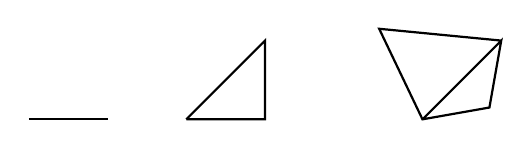
\begin{tikzpicture} \draw [thick] (0,0) to (1,0) ;

\draw [thick] (2,0) to (3,0) to (3,1) to (2,0);

\draw  [thick] (5,0) to (6,1) to (5.85,.15) to (5,0) to (4.45,1.15) to (6,1); \end{tikzpicture} 
\par\end{center}


These are fundamental to algebraic topology.

\item Presheaf categories are closely connected to categories of sheaves,
which are also topoi. Sheaves are fundamental to algebraic geometry. 
\end{enumerate}
\end{example} 


\section{Symmetric Monoidal Categories}


\subsection{Guest lecture by Christina Osborne}
\begin{quote}
A category theorist is sort of like a sociologist. He looks at mathematical
objects - he doesn't pry it open and see how it works - but sees how
it behaves in relation to all other things. 

- Chris Heunen
\end{quote}

\subsubsection{What is a Monoidal Category?}

\begin{defn} A $\emph{monoid}$ is a nonempty set $G$ together with
a binary operation on $G$ which is:
\begin{itemize}
\item associative: $(xy)z=x(yz)$ ~~~$\forall$ $x,y,z\in G$ 
\item and contains a (two-sided) identity element $e\in G$ such that $xe=ex=x$
~~~$\forall$ $x,y,z\in G$
\end{itemize}
\begin{rem} i.e. take the definition of a group and drop the requirement of inverses \end{rem}

\end{defn}

\begin{defn} A $\emph{monoidal category}$ is a category $\mathbf{C}$
which is equipped with:
\begin{enumerate}
\item A tensor product functor $\otimes:\mathbf{C\times C\to C}$ where
the image of a pair of objects $(x,y)$ is denoted by $x\otimes y$.
\item A $\emph{unit object}$ $I$. 
\item For every $x,y,z\in Ob(\mathbf{C})$, and associativity isomorphism
$a_{x,y,z}:(x\otimes y)\otimes z\to x\otimes(y\otimes z)$, natural
in the objects $x$, $y$, and $z$. 
\item For every $x\in Ob(\mathbf{C})$, a left unit isomorphism $\ell_{x}:I\otimes X\to X$
and a right unit isomorphism $r_{x}:x\otimes I\to x$, both natural
in $x$.
\end{enumerate}
We further assume the following diagrams commute for any objects $w$,
$x$, $y$, and $z$:
\begin{itemize}
\item the $\textbf{pentagon identity}$:
\end{itemize}
\begin{center}\begin{tikzcd} && ((w \otimes x) \otimes y) \otimes z \arrow[rrdd, "a_{w \otimes x,y,z}"] \arrow[lldd, "a_{w,x,y} \otimes id_{z}" swap] \\\\ (w \otimes (x \otimes y)) \otimes z \arrow[ddd, "a_{w,x \otimes y,z}" swap] &&&& (w \otimes x) \otimes (y \otimes z) \arrow[ddd, "a_{w,x,y \otimes z}"] \\\\\\ w \otimes ((x \otimes y) \otimes z) \arrow[rrrr, "id_{z} \otimes a_{x,y,z}" swap] &&&& w \otimes (x \otimes (y \otimes z)  \end{tikzcd}\end{center}
\begin{itemize}
\item the $\textbf{triangle identity}$:
\end{itemize}
\begin{center}\begin{tikzcd} \\\\ (x \otimes I) \otimes y \arrow[rr, "a_{x,I,y}"] \arrow[rddd, "r_{x} \otimes id_{y}" swap] && x \otimes (I \otimes y) \arrow[lddd, "id_{x} \otimes \ell _{y}"] \\\\\\ & x \otimes y \end{tikzcd} \end{center}

\begin{rem} When we want to emphasize the tensor product and unit,
we denote a monoidal category by $(\mathbf{C},\otimes,I)$. \end{rem}

\end{defn}

\begin{example}$(\mathbf{Set},\times,\{\bullet\})$ \end{example}

\begin{example} $(\mathbf{Set},\coprod,\{\emptyset\})$\end{example}

\begin{example}$(\mathbf{Grp},\times,\{e\})$ \end{example}

\begin{example} $(\mathbf{Hilb},\otimes,\mathbb{C})$, where the
category $\mathbf{Hilb}$ has Hilbert spaces as objects and short
linear maps (linear maps of norm at most 1) as morphisms. \end{example}

\begin{flushleft}
Why is $a_{x,y,z}:(x\otimes y)\otimes z\to x\otimes(y\otimes z)$
an isomorphism and not an equality? Let's consider the example $(\mathbf{Set},\times,\{\bullet\})$
:
\[
(X\times Y)\times Z=\{(w,z)\mid w\in X\times Y,\,z\in Z\}=\{((x,y),z)\mid x\in X,\,y\in Z,\,z\in Z\}
\]
\[
X\times(Y\times Z)=\{(x,w)\mid x\in X,\,w\in Y\times Z=\{(x,(y,z))\mid x\in X,\,y\in Y,\,z\in Z\}
\]

\par\end{flushleft}

\begin{flushleft}
These sets are $\emph{not}$ equal - but we can easily construct an
isomorphism. 
\par\end{flushleft}

\begin{example} How can we take a monoid~$G$ and construct a monoidal
category? First we need a category $\mathbf{C}$: 
\begin{itemize}
\item objects: elements of $G$. 
\item morphisms: identity morphisms.
\end{itemize}
We get a monoidal category $(\mathbf{C},\bullet,e)$ where $\bullet$
is the binary product of $G$ and $e$ is the identity element of
$G$.\end{example}

\begin{flushleft}
$\textbf{Note:}$ In general:
\par\end{flushleft}
\begin{itemize}
\item If $\mathbf{C}$ has products, we get a monoidal category $(\mathbf{C},\times,1)$.
\item If $\mathbf{C}$ has coproducts, we get a monoidal category $(\mathbf{C},+,0)$.
\end{itemize}
\begin{defn} A monoidal category $(\mathbf{C},\otimes,I)$ is $\emph{symmetric}$
if it additionally is equipped with an isomorphism $s_{x,y}:x\otimes y\to y\otimes x$
for any objects $x$ and $y$ of $\mathbf{C}$, natural in $x$ and
$y$, such that the following diagrams commute for all objects $x$,
$y$, and $z$:

\begin{center}\begin{tikzcd} \\ & (x \otimes y) \otimes z \arrow[ldd, "a_{x,y,z}" swap] \arrow[rr, "s_{x,y} \otimes id_{z}"] && (y \otimes x) \otimes z \arrow[rdd, "a_{y,x,z}"]  \\\\ x \otimes (y \otimes z) \arrow[ddr, "s_{x,y \otimes z}" swap] &&&& y \otimes (x \otimes z) \arrow[ddl, "id_{y} \otimes s_{x,z}"] \\\\ & (y \otimes z) \otimes x \arrow[rr, "a_{y,z,x}" swap] && y \otimes (z \otimes x)  \end{tikzcd}\end{center}

\begin{center}\begin{tikzcd} \\\\ x \otimes I \arrow[rr, "s_{x,I}"] \arrow[rddd, "r_{x}" swap] && I \otimes x \arrow[lddd, "\ell _{x}"] \\\\\\ & x \end{tikzcd} \end{center}

\begin{center}\begin{tikzcd} \\\\ x \otimes y \arrow[rr, "s_{x,y}"] \arrow[rddd, "id_{x \times y}" swap] && y \otimes x \arrow[lddd, "s_{y,x}"] \\\\\\ & x \otimes y \end{tikzcd} \end{center}

\end{defn}

\begin{flushleft}
Most of the examples of monoidal categories we have talked about are
symmetric. So what's an example of a monoidal category that is not
symmetric?
\par\end{flushleft}

\begin{example} Let $R$ be a non-commutative ring. The category
$R$-$R$-bimodules with $_{R}\otimes_{R}$ as the tensor and $R$
as the unit is an example of a monoidal category that is not symmetric.
\end{example}

$\textbf{Note:}$ Let $(\mathbf{C},\bullet,e)$ be the monoidal category
given by the monoid $G$. If $G$ is an abelian group, then $(\mathbf{C},\bullet,e)$
is symmetric.


\subsubsection{Going back to the definition of a symmetric monoidal category...}

Q: Why is the hexagon commuting diagram sufficient?
\begin{itemize}
\item There are 6 different ways to order 3 elements.
\item There are 2 ways of associating 3 elements.
\item So there are 12 possibilities (we would expect all of these to be
isomorphic).
\end{itemize}
A: repeat!

\begin{center}\begin{tikzcd} \\ & (x \otimes y) \otimes z \arrow[ldd] \arrow[rr] && (y \otimes x) \otimes z \arrow[rdd]  \\\\ x \otimes (y \otimes z) \arrow[ddr] &&&& y \otimes (x \otimes z) \arrow[ddl] \\\\ & (y \otimes z) \otimes x \arrow[rr, "a_{y,z,x}" swap] && y \otimes (z \otimes x)  \end{tikzcd}\end{center}

\begin{center}\begin{tikzcd} \\ & (y \otimes z) \otimes x \arrow[ldd] \arrow[rr] && (z \otimes y) \otimes x \arrow[rdd]  \\\\ y \otimes (z \otimes x) \arrow[ddr] &&&& z \otimes (y \otimes x) \arrow[ddl] \\\\ & (z \otimes x) \otimes y \arrow[rr] && z \otimes (x \otimes y)  \end{tikzcd}\end{center}

\begin{center}\begin{tikzcd} \\ & (z \otimes x) \otimes y \arrow[ldd] \arrow[rr] && (x \otimes z) \otimes y \arrow[rdd]  \\\\ z \otimes (x \otimes y) \arrow[ddr] &&&& x \otimes (z \otimes y) \arrow[ddl] \\\\ & (x \otimes y) \otimes z \arrow[rr] && x \otimes (y \otimes z)  \end{tikzcd}\end{center}


\section{Week 10}


\subsection{The subobject classifier in Graph$ $}

This is some graph $\Omega$ such that subgraphs $A$ of any graph
$X$ corresponds to morphisms of graphs $\chi:X\to\Omega$ in such
a way that

\begin{center}
\begin{center}\begin{tikzcd} A \arrow[r,"!A"] \arrow[d,"i",swap ]& 1 \arrow[d,"t" ] \\ X \arrow[r," \chi " ] & \Omega \end{tikzcd}\end{center}
\par\end{center}

is a pullback. $\Omega$ looks like this:

\begin{center}\begin{tikzcd} \bullet \arrow[loop left, dotted, "OUT"] \arrow[loop above, "IN"] \arrow[r, dotted, bend left] & \circ \arrow[loop right, dotted, "OUT", very near start] \arrow[l,bend left, dotted]  \end{tikzcd}\end{center} 

The terminal graph, \textquotedbl{}$\mathbf{1}$\textquotedbl{}, looks
like this: \begin{tikzcd} \bullet \arrow[loop] \end{tikzcd} \\
 The purple subgraph of $\Omega$ is a copy of $\mathbf{1}$ (it's
isomorphic to $\mathbf{1}$). We get this from the morphism $t:1\to\Omega$
which you have in any topos. A vertex or edge of $X$ will be mapped
to this subgraph of $\Omega$ iff it's true that the vertex or edge
is in A.\\
 The most important basic properties of topoi:

\begin{prop} A topos has finite colimits, meaning it has colimits
of finite-sized. \end{prop} \begin{prop} Any morphism $f:X\to Y$
in a topos has an epi-mono factorization i.e. there exists an epimorphism
$p:X\to A$ and a mono $i:A\to Y$ making this triangle commute: 

\begin{center}
\begin{tikzcd} X \arrow[rr,"f"] \arrow[dr,"p" swap]& & Y \\ & A \arrow[ur,"i" swap] & \end{tikzcd}
\par\end{center}

\end{prop}

\begin{prop} In a topos, the epi-mono factorization of any morphism
$f:X\to Y$ is unique up to a unique isomorphism. Given two epi-mono
factorization: 

\begin{center}
\begin{tikzcd} X \arrow[ddr,"p'", bend right, swap] \arrow[rr,"f"] \arrow[dr,"p" swap]& & Y \\ & A \arrow[d,dashrightarrow] \arrow[ur,"i" swap] & \\ & A' \arrow[uur,"i'", bend right, swap]& \end{tikzcd} 
\par\end{center}

there exists a unique isomorphism $g:A\to A'$ making the resulting
diagram commute. \end{prop}

\begin{example} In $\mathbf{Set}$, we have an epi-mono factorization 

\begin{center}
\begin{tikzcd}  X \arrow[rr,"f"] \arrow[dr,"p" swap]& & Y \\ & im(f) \arrow[ur,"i" swap] & \end{tikzcd}  
\par\end{center}

where $im(f)=\{y\in Y:y=f(x)$ for some $x\in X\}$, $i:im(f)\to Y$
is the inclusion and $p:X\to im(f)$ is the obvious function $p(x)=f(x)\in im(f)$.
\end{example} So: \begin{defn} Given an epi-mono factorization: 

\begin{center}
\begin{tikzcd}  X \arrow[rr,"f"] \arrow[dr,"p" swap]& & Y \\ & A \arrow[ur,"i" swap] & \end{tikzcd} 
\par\end{center}

we call $A$ \textquotedbl{}the\textquotedbl{} image of $f$ (it's
unique up to isomorphism) and denote it as im(f). \end{defn} Generalize
$\subseteq,\cap,\cup$ to any topos, henceforth suppose $\mathbf{C}$
is a topos. \begin{defn} Given $X\in\mathbf{C}$, define $Sub(X)$
to be the set of all subobjects of X:equivalence classes of monomorphisms
$i:A\to X$, where $i:A\to X$ and $j:A\to X$ are equivalent iff
there exists an isomorphism $g:A\to B$ so that: 

\begin{center}
\begin{tikzcd}[column sep=small]  A \arrow[rr,"i"] \arrow[dr,"g" swap]& & X \\ & B \arrow[ur,"j" swap] & \end{tikzcd} 
\par\end{center}

commutes. \end{defn}

\begin{note} $Sub(X)\cong hom(X,\Omega)$ since $\Omega$ is the
subobject classifier. \end{note}

\begin{prop} $Sub(X)$ is a poset where we say the equivalence class
of $i:A\to X$ is contained in (or $\subseteq$) the equivalence class
of $j:B\to X$ if there exists $f:A\to B$ making this commute: 

\begin{center}
\begin{tikzcd}[column sep=small]  A \arrow[rr,"i"] \arrow[dr,"f" swap]& & X \\ & B \arrow[ur,"j" swap] & \end{tikzcd} 
\par\end{center}

(Note: $f$ must be a monomorphism, and it's unique) \end{prop}

\begin{proof} Need to check:
\begin{itemize}
\item If $[i]\subseteq[j]$ and $[j]\subseteq[k]$, then $[i]\subseteq[k]$
\end{itemize}
\begin{center}
\begin{tabular}{ccccc}
\begin{tikzcd} A \arrow[r,"i"] \arrow[d,"f" swap] & X \\ B \arrow[r,"g" swap] \arrow[ur, "j" swap] & C \end{tikzcd} &  & gives &  & \begin{tikzcd} A \arrow[r,"i"] \arrow[d,"g \circ f" swap] & X \\ C \arrow[ur, "k" swap] \end{tikzcd}\tabularnewline
\end{tabular}
\par\end{center}
\begin{itemize}
\item $[i]\subseteq[i]$ - easy
\item If $[i]\subseteq[j]$ and $[j]\subseteq[i]$, then $[i]=[j]$
\end{itemize}
\begin{center}
\begin{tabular}{ccccc}
\begin{tikzcd} A \arrow[r,"i"] \arrow[d,"f" swap] & X \\ B \arrow[ur, "j" swap]\end{tikzcd} &  &  &  & \begin{tikzcd} A \arrow[r,"i"] & X \\ B \arrow[u, "g"] \arrow[ur, "k" swap] \end{tikzcd}\tabularnewline
\end{tabular}
\par\end{center}

\begin{flushleft}
To show $[i]=[j]$, it suffices to show:
\par\end{flushleft}

\begin{center}
\begin{tabular}{ccccc}
\begin{tikzcd} A \arrow[dr,"i"] \arrow[d,"f" swap] \\ B \arrow[r, "j"] \arrow[d,"g" swap] & X \\ A \arrow[ur, "i" swap] \end{tikzcd} &  &  &  & \begin{tikzcd} B \arrow[dr,"j"] \arrow[d,"g" swap] \\ A \arrow[r, "i"] \arrow[d,"f" swap] & X \\ B \arrow[ur, "j" swap] \end{tikzcd}\tabularnewline
\end{tabular}
\par\end{center}

\begin{flushleft}
commute, so $i\circ g\circ f=i\circ1_{A}$ and $j\circ f\circ g=j\circ1_{B}$,
and since $i$ and $k$ are monic, they're left cancellable: $g\circ f=1_{A}$
and $f\circ g=1_{B}$ 
\par\end{flushleft}

\end{proof}

Next time we'll define $U$ for subobjects, and this makes $Sub(X)$,
which is a poset (hence a category), into a category with coproducts:
$\cup$ is the coproduct in $Sub(X)$. Similarly, $\cap$ is the product
in the category $Sub(X)$.


\subsection{Set Theory, Topos, and Logic}

In $\mathbf{Set}$, every subset of $X\in\mathbf{Set}$ corresponds
to a predicate on elements of $X$:

\begin{center}
\begin{tabular}{ccc}
$\chi:X\to\{T,F\}$ &  & i.e. a characteristic function\tabularnewline
\end{tabular} 
\par\end{center}

\begin{flushleft}
$\chi$ determines a subset $A\mbox{\ensuremath{\subseteq}}X$ via:
\[
A=\{x\in X\mid\chi(x)=T\}
\]

\par\end{flushleft}

\begin{flushleft}
and conversely, any subset $A\subseteq X$ determines $\chi:X\to\{T,F\}$
via:
\[
\chi(x)=\begin{cases}
T & x\in A\\
F & x\notin A
\end{cases}
\]

\par\end{flushleft}

\begin{flushleft}
In a topos, we get a similar bijection between $Sub(X)$ and $Hom(X,\Omega)$.
The concepts of $\cup$ and $\cap$ for subsets correspond to the
operations of $\land$ and $\lor$ on predicates.
\[
\{x\in X\mid\chi(x)=T\}\cup\{x\in X\mid\varphi(x)=T\}=\{x\in X\mid(\chi\lor\varphi)(x)=T\}
\]

\par\end{flushleft}

\begin{flushleft}
and similarly for $\cap$ and $\land$. 
\par\end{flushleft}

\begin{prop} In $\mathbf{Set}$, $Sub(X)$ for $X\in\mathbf{Set}$
is a poset via $\subseteq$, and thus a category where there exists
a unique morphism from $A$ to $B$ if and only if $A\subseteq B$
$(A,B\subseteq X)$. In this category $A\cap B$ is the product of
$A$ and $B$, and $A\cup B$ is the coproduct.\end{prop}

\begin{proof} We have 

\begin{center}\begin{tikzcd}[column sep=small] & A \cap B \arrow[dr, " \subseteq "] \arrow[dl, " \subseteq " swap] \\ A && B \end{tikzcd}\end{center}

\begin{flushleft}
and this cone is universal:
\par\end{flushleft}

\begin{center}\begin{tikzcd}[column sep=small] & Q \arrow[d, dotted, " \exists ! \psi "] \arrow[ddl,bend right, " \subseteq " swap] \arrow[ddr, bend left, " \subseteq "] \\ & A \cap B \arrow[dr, " \subseteq "] \arrow[dl, " \subseteq " swap] \\ A && B \end{tikzcd}\end{center}

\begin{flushleft}
which is true since $Q\subseteq A$, $Q\subseteq B$ $\implies$ $Q\subseteq A\cap B$.
\par\end{flushleft}

\end{proof}

In fact, in $\mathbf{Set}$, $Sub(X)$ has all finite limits and all
finite colimits! A category has all finite limits if an only if it
has:
\begin{itemize}
\item binary products
\item a terminal object
\item equalizers
\end{itemize}
$Sub(X)$ has binary products $(\cap)$, a terminal object ($X$,
since $A\subseteq X$ for all $A\in Sub(X)$) and equalizers: \begin{tikzcd} B \arrow[r, shift left, "f"] \arrow[r,shift right, "g" swap] & C \end{tikzcd}
in any poset is really \begin{tikzcd} B \arrow[r, shift left, "f"] \arrow[r,shift right, "f" swap] & C \end{tikzcd},
and the equalizer is:

\begin{center}\begin{tikzcd} B \arrow[r,"i"] & B \arrow[r, shift left, "f"] \arrow[r,shift right, "f" swap] & C \end{tikzcd}\end{center}
so equalizers exist in any poset. Similarly in $\mathbf{Set}$, $Sub(X)$
has all finite colimits because it has:
\begin{itemize}
\item binary coproducts
\item an initial object
\item coequalizers
\end{itemize}
The binary coproduct of $A$ and $B$ is $A\cup B$, the initial object
is $\emptyset$ (since $\emptyset\subseteq A$ for all $A\in Sub(X)$),
and coequalizers (which exist in any poset: just turn arrows around
in argument for equalizers).

\begin{defn} A $\emph{lattice}$ is a poset with all finite limits
and colimits. \begin{rem} This is equivalent to other more popular
definitions, though some evil people don't demand the initial and
terminal object. \end{rem} \end{defn}

In fact we have:

\begin{center}
\begin{tabular}{|c|c|c|}
\hline 
SET THEORY & LOGIC & CATEGORY THEORY\tabularnewline
\hline 
\hline 
$\cap$ & $\land$ & binary product\tabularnewline
\hline 
$X$ (the whole set) & $T$  & terminal object\tabularnewline
\hline 
$\cup$  & $\lor$ & binary coproduct\tabularnewline
\hline 
$\emptyset$ & $F$ & initial object\tabularnewline
\hline 
$B\cup A^{c}$ & $Q\lor\lnot P$ or ``P implies Q'' & exponentiation\tabularnewline
\hline 
\end{tabular}
\par\end{center}

\begin{flushleft}
$\textbf{Note}$: 
\[
X=\{x\in X\mid T=T\}
\]
\[
\emptyset=\{x\in X\mid F=T\}
\]

\par\end{flushleft}

\begin{flushleft}
In fact, the poset $Sub(X)$ is cartesian closed. In general, this
means:
\[
Hom(B\times C,D)\cong Hom(B,D^{C})
\]

\par\end{flushleft}

\begin{flushleft}
but for $Sub(X)$, being a poset, these sets either have $0$ elements
or $1$ element. Also, the product is the intersection. So this says:
\par\end{flushleft}

\begin{center}
\begin{tabular}{ccc}
$B\cap C\subseteq D$ & if and only if & $B\subseteq D\cup C^{c}$\tabularnewline
\end{tabular} 
\par\end{center}

\begin{flushleft}
or in terms of logic:
\par\end{flushleft}

\begin{center}
\begin{tabular}{ccc}
$P\land Q\implies R$  & if and only if & $P\implies R\lor\lnot Q$ \tabularnewline
\end{tabular} 
\par\end{center}

\begin{theorem} In any topos, for any object $X$ the poset $Sub(X)$
is a $\emph{Heyting algebra}$: it's a poset that has finite limits,
finite colimits, and is cartesian closed. \begin{rem} i.e. it's a
Cartesian closed lattice \end{rem}\end{theorem}

\begin{proof} Given two subobjects of $X$, $[i]$ and $[j]$, we
want to form $[i]\cap[j]$ and $[i]\cup[j]$. Taking the pullback
gives us the intersection:

\begin{center}\begin{tikzcd} A \cap B \arrow[dr, "i \circ f", "j \circ g" swap] \arrow[d, "f" swap] \arrow[r, "g"] & B \arrow[d, "j"] \\ A \arrow[r, "i"] & X \end{tikzcd}\end{center}

\begin{flushleft}
Since this is a pullback and $i$,$j$ are monic, then $f$,$g$,
must be monic too (monics pullback to monics). This implies $i\circ f=j\circ g$
is monic too, so we get a new subobject of $X$, which is $[i]\cap[j]$.
For unions, we start with the product: 
\par\end{flushleft}

\begin{center}\begin{tikzcd} A + B \arrow[dr,"\exists ! \psi "] & B \arrow[l, "g" swap] \arrow[d, "j"] \\ A \arrow[r, "i"] \arrow[u, "f"] & X \end{tikzcd}\end{center}

\begin{flushleft}
where we get $\psi$ from the universal property of the coproduct.
But $\psi$ need not be monic, so do the epi-mono factorization:
\par\end{flushleft}

\begin{center}\begin{tikzcd} A + B \arrow[dr,"p" swap] \arrow[rr, "\psi "] && X \\ & im\psi \arrow[ru, "k" swap] \end{tikzcd}\end{center}

\begin{flushleft}
where $p$ is epic and $k$ is monic. $k$ gives a new subobject of
$X$, which is $[i]\cup[j]$. 
\par\end{flushleft}

\end{proof}


\subsection{Where does topos theory go from here?}

Many directions.... e.g.:
\begin{itemize}
\item Using the ``Mitchell-Benabov language'', we can reason inside any
topos:
\end{itemize}
\begin{flushleft}
We can write things like:
\[
\{x\in A\cap B\mid\forall y\in Y\,\,\exists z\in Z\,\,f(x,z)=y\}
\]

\par\end{flushleft}

\begin{flushleft}
and prove things about them using the logic internal to the topos,
and ``generalized elements''.
\par\end{flushleft}
\begin{itemize}
\item There are also maps between topoi:
\end{itemize}
\begin{center}\begin{tikzcd} C \arrow[r, bend left] & D \arrow[l, bend left] \end{tikzcd}\end{center}

\begin{flushleft}
consisting of certain nice adjunctions. These maps are called ``geometric
morphisms''. There's a topos called $\mathbf{Th(Grp)}$ - ``the
theory of groups'', and then a geometric morphism from some other
topos $\mathbf{C}$ to $\mathbf{Th(Grp)}$ is the same as a group
object in $\mathbf{C}$. This idea works for lots of concepts, not
just the concept of a group.
\par\end{flushleft}
\end{document}
